%%
%% Topography-Consistent RF Propagation Modeling
%% Target: IEEE Access -- classe oficial da revista (ieeeaccess.cls)
%%
\documentclass{ieeeaccess}

%% --- Pacotes ---
%% A classe ieeeaccess (\LoadClass{IEEEtran}) ja carrega: color e hyperref.
%% NAO recarregue hyperref aqui: a classe o injeta com [hidelinks].
\usepackage{cite}
\usepackage{amsmath,amssymb,amsfonts}
\usepackage{algorithm}
\usepackage{algorithmic}
\usepackage{graphicx}
\usepackage{textcomp}
\usepackage{booktabs}
\usepackage{multirow}
\usepackage{array}
\usepackage{float}
\usepackage{subcaption}
\usepackage{siunitx}
% siunitx não define \bel por padrão; isto habilita \SI{...}{\deci\bel} (dB)
\DeclareSIUnit\bel{B}
\providecommand{\pend}[1]{\textcolor{red}{[PENDING: #1]}}
\usepackage{url}
\graphicspath{{figures/}{pic/}{./}}

\begin{document}

%% --- Cabecalho de publicacao IEEE Access (preenchido pela revista) ---
\history{Date of publication xxxx 00, 0000, date of current version xxxx 00, 0000.}
\doi{XX.XXXX/ACCESS.YYYY.DOI}

\title{Physics-Informed Multi-Target RF Field Reconstruction over Heterogeneous Terrain Graphs under Spatially Blocked Evaluation}

\author{
\uppercase{L. F. C. Seelig}\authorrefmark{1,2},
\uppercase{and R. M. Salles}\authorrefmark{1,3}}

\address[1]{Postgraduate Program in Defense Engineering (PGED), Military Institute of Engineering (IME), Rio de Janeiro, Brazil. 
}
\address[2]{Military Science Laboratory, Brazilian Army Command and General Staff College (ECEME), Brazil (e-mail: seelig.felipe@eb.mil.br)}
\address[3]{Center for Innovation and Research in Business Sciences and Information Systems (CIICESI), ESTG, Polytechnic of Porto, Portugal (e-mail: rmo@estg.ipp.pt)}

%% Informacao de fomento/agradecimento (opcional). Descomente e preencha se houver:
%% \tfootnote{This work was supported in part by ...}

%\markboth{Seelig \headeretal: Physics-Consistent Multi-Target RF Field Reconstruction over Heterogeneous Terrain Graphs}
%{Seelig \headeretal: Physics-Consistent Multi-Target RF Field Reconstruction over Heterogeneous Terrain Graphs}

\markboth{Seelig \& Salles: Physics-Informed Multi-Target RF Field Reconstruction over Heterogeneous Terrain Graphs}
{Seelig \& Salles: Physics-Informed Multi-Target RF Field Reconstruction over Heterogeneous Terrain Graphs}


\corresp{Corresponding author: R. M. Salles (e-mail: salles@ime.eb.br).}

\begin{abstract}
Empirical models like FSPL, Okumura--Hata, and COST\,231 lose accuracy where terrain, vegetation, and urban fabric shape sub-kilometer propagation beyond coarse categories, and the evaluation partition changes what a comparison supports. GNN-RF, a heterogeneous GATv2 graph neural network, is trained on $12.96 \times 10^6$-node terrain graphs from four S\~{a}o Paulo cities to reconstruct path loss, RSSI, and coverage, with a physics-constrained decoder and four loss regularizers: free-space floor, monotonicity, variance, and NDVI sign. Under spatial blocking (80~runs), GNN-RF's all-node RSSI MAE is \SI{0.395}{\deci\bel} (95\% CI [\num{0.309}, \num{0.480}]), on average \SI{0.746}{\deci\bel} below each cell's best calibrated empirical model (paired $p{=}2.59\times10^{-4}$), winning 15 of 16 cells. Over the 17.04\% valid-target subset, its MAE is \SI{2.012}{\deci\bel} (cell mean, Lins~Q1 included), against \SI{4.362}{\deci\bel} for that model, ahead in 12 of 16 cells. GNN-RF's all-node MAE is \SI{0.247}{\deci\bel} below a graph-free control matched in nominal parameters (city-level interval crossing zero, $p{=}0.205$); on valid-target nodes, GNN-RF and a node-wise RadioUNet adaptation with only antenna-to-terrain graph relations are 0.727 and \SI{1.5060}{\deci\bel} below that control, and their difference, like the effect of retraining without penalties, is inconclusive relative to the pre-specified margin. Uncertainty quantification fails a pre-specified joint coverage criterion: MC Dropout qualifies in 3 of 16 cells, split-conformal in 1, and a residual-based baseline in 2. Labels come from a deterministic propagation generator, so errors measure fidelity to simulated references, not physical-world prediction error.
\end{abstract}


\begin{keywords}
RF propagation modeling, graph neural networks, physics-informed learning, heterogeneous graphs, topography, transfer learning, uncertainty quantification
\end{keywords}

\titlepgskip=-15pt

\maketitle

\section{Introduction}
\label{sec:introduction}
%% ====================================================================

\PARstart{S}{ub-kilometer} radio frequency (RF) propagation over morphologically heterogeneous terrain challenges the assumptions of classical coverage models. Free-Space Path Loss (FSPL), Okumura--Hata~\cite{hata1980empirical}, and COST\,231~\cite{cost231} estimate attenuation through closed-form expressions derived from large-scale measurements, but reduce local relief, vegetation, and urban structure to a limited set of terrain categories~\cite{vasudevan2024machine}. Local ground cover causes location variability over areas of a few hundred meters~\cite{itu1546}, shadow fading is spatially correlated~\cite{tr38901}, and vegetation and buildings cause large-scale fading~\cite{thrane2020model}. Coverage prediction depends on path-loss estimates~\cite{vasudevan2024machine}, yet conventional empirical methods cannot provide location-specific, high-fidelity predictions in complex propagation environments~\cite{yapar2024overview}.

This limitation is especially relevant in Brazil, where the vegetated suburban and rural environments with tropical species differ from the temperate-clime conditions on which most models of propagation through vegetation are based~\cite{silva2018propagation}, and where Okumura--Hata departs from field measurements of sub-GHz links in the Amazon~\cite{lima2024lora}. Elsewhere, at 900~MHz in Cartagena, Spain, classical empirical models err well above models conditioned on local geospatial descriptors~\cite{lorentelpez2026machine}, so expanding sub-GHz coverage into suburban areas calls for site-specific predictions beyond what closed-form models can provide.

Learned radio-map estimators~\cite{levie2021radiounet,zhang2023rme,shibli2024data} improve over empirical models but still face structural limitations for multi-city deployment (Section~\ref{sec:related_work}). Grid-based models cannot natively represent irregular terrain sampling; physics priors often stop at a path-loss floor and omit vegetation or terrain-gradient effects; evaluations are commonly limited to a single city or synthetic scenarios; and comparisons across architectures frequently use different feature sets, losses, and optimization schedules. These limitations make it difficult to separate gains due to terrain representation from gains due to training design, especially without identical-treatment comparisons and anti-leakage controls.

GNN-RF addresses these gaps by operating natively on the heterogeneous terrain graph instead of on a rasterized proxy of it. Each city quadrant becomes a graph of $12.96 \times 10^6$~nodes with three edge types and 18 topographic and spectral features, encoded by a multi-head GATv2 stack and decoded into a five-channel RF output by a physics-constrained head. The output activations bound each channel, and the loss penalizes departures from free-space bounds, distance--attenuation monotonicity, variance preservation, and NDVI sign consistency.

Training follows a sequential transfer protocol across geographic quadrants and is evaluated over 80~runs under spatially blocked partitions spanning four cities in S\~{a}o Paulo state, complemented by cross-city transfer. Because every target label is produced by a fully specified deterministic propagation generator (detailed in the Supplementary Material) rather than measured in the field, the reported accuracy bounds reconstruction fidelity relative to simulation-derived references, not physical-world prediction error. Evaluation design matters for such a target: on the same reference field, a nearest-neighbor predictor errs roughly an order of magnitude more under the spatially blocked split used throughout this work than under a random node split, in every city (Section~\ref{sec:eval_protocol}).

The contributions of this work are fivefold. We design a heterogeneous GNN that pairs a multi-head GATv2 encoder with a physics-constrained decoder that jointly predicts total path loss, RSSI, and coverage, supervising vegetation and terrain-diffraction attenuation against the corresponding components of the reference generator. We formulate a composite physics-informed objective that joins a Huber regression term with four domain regularizers: an FSPL-floor penalty, distance--attenuation monotonicity, variance preservation, and NDVI sign consistency; we test their contribution by retraining the model in two arms of 80 runs, one without any of the four terms and one without the monotonicity term alone. We define a sequential transfer-learning protocol over quadrants (Q1$\to$Q4) and test it against training every quadrant from scratch.

We evaluate GNN-RF under a spatially blocked protocol that limits spatial leakage between training and test~\cite{roberts2017cross}, a split-related form of data leakage~\cite{apicella2025don}, against calibrated empirical models, a graph-free control matched in nominal parameters, edge-relation ablations, and, as a learned baseline trained under the same blocked protocol with the same loss and output decoder, an in-house, node-wise adaptation of RadioUNet~\cite{levie2021radiounet}. We evaluate Monte Carlo Dropout~\cite{gal2016dropout} uncertainty across all 16~city--quadrant pairs at five nominal levels, with split-conformal and residual-based comparisons.


%% ====================================================================
\section{Theoretical Foundation and Related Work}
\label{sec:related_work}
%% ====================================================================

Heterogeneous message passing supplies an inductive bias that supports a multi-relation terrain graph, since it assigns separate parameters to each relation type instead of forcing one rule across every interaction. A heterogeneous graph is the tuple $\mathcal{G} = (\mathcal{V}, \mathcal{E}, \mathcal{R}, \phi, \psi)$, with node set $\mathcal{V}$, edge set $\mathcal{E} \subseteq \mathcal{V} \times \mathcal{V}$, relation types $\mathcal{R}$, and type-assignment maps $\phi: \mathcal{V} \to \mathcal{T}_V$ and $\psi: \mathcal{E} \to \mathcal{T}_E$~\cite{zhai2025heterogeneous}. Over such graphs the Graph Attention Network~\cite{velickovic2018graph} learns adaptive neighbor weights, and GATv2~\cite{brody2022attentive} computes dynamic attention, whereas the original formulation computes only static attention:
\begin{equation}
\alpha_{ij} = \frac{\exp\!\bigl(\mathbf{a}^\top \mathrm{LeakyReLU}(\mathbf{W}[\mathbf{h}_i \| \mathbf{h}_j \| \mathbf{e}_{ij}])\bigr)}{\sum_{k \in \mathcal{N}(i)} \exp\!\bigl(\mathbf{a}^\top \mathrm{LeakyReLU}(\mathbf{W}[\mathbf{h}_i \| \mathbf{h}_k \| \mathbf{e}_{ik}])\bigr)}
\label{eq:gatv2}
\end{equation}
where $\mathbf{W}$ is a learnable weight matrix, $\mathbf{a}$ the attention vector, $\mathbf{h}_i$ the node embedding, $\mathbf{e}_{ij}$ the edge feature, and $\|$ denotes concatenation; $K$ parallel heads are concatenated before projection, as in GAT~\cite{velickovic2018graph}. Relation-specific message passing, built on the scheme in which each node sums messages from its neighbors and then updates its state~\cite{gilmer2017neural}, composes these per-relation attention maps into a single node update,
\begin{equation}
\mathbf{h}_i^{(\ell+1)} = \sigma\!\Biggl(\sum_{r \in \mathcal{R}} \sum_{j \in \mathcal{N}_r(i)} \alpha_{ij}^{(r)} \mathbf{W}_r^{(\ell)} \mathbf{h}_j^{(\ell)}\Biggr)
\label{eq:hetero_mp}
\end{equation}
with $\mathbf{W}_r^{(\ell)}$ and $\alpha_{ij}^{(r)}$ the transformation and attention weights for relation $r$ at layer $\ell$ and $\sigma$ a nonlinearity, so that propagation, connectivity, and range relations each learn a distinct interaction rule.

Classical propagation models buy closed-form tractability at the cost of morphological resolution. Free-space path loss follows from the free-space transmission formula~\cite{friis1946note}; expressed in decibels as a function of distance and frequency, it sets the theoretical attenuation floor,
\begin{equation}
L_{\text{FSPL}} = 20\log_{10}(d) + 20\log_{10}(f) + 32.44 \quad [\text{dB}]
\label{eq:fspl}
\end{equation}
with $d$ in km and $f$ in MHz; Okumura--Hata adds empirical corrections for antenna height~\cite{hata1980empirical,itu529} and for suburban and open areas relative to the urban formula~\cite{hata1980empirical}, and COST\,231~\cite{cost231} carries the same scheme into the 1500--2000~MHz band. Terrain-aware standards go further: \mbox{ITU-R} P.1546~\cite{itu1546} integrates elevation profiles for point-to-area field strength, and \mbox{ITU-R} P.833~\cite{itu833} models canopy attenuation. Even so, the Okumura--Hata and COST\,231 models treat two environments alike whenever they fall into the same propagation category, which limits their accuracy at a given location~\cite{yapar2024overview}, and a first analysis reports that high-resolution terrain and land-use data improve ITU-R P.1812 predictions where small obstacles block the signal~\cite{hamada2025enhancing}.

Learned estimators raise accuracy over empirical models, but each line of work solves only part of the terrain problem. RadioUNet~\cite{levie2021radiounet} treats path loss as image translation on a 2D grid and was the public baseline of a challenge on path-loss radio maps from city maps and transmitter locations~\cite{yapar2023the}. Radio-map estimation from sparse measurements~\cite{feng2025recent} keeps that grid in its image-based methods: completion autoencoders take the measurements with a mask of their grid locations and the building map, as surveyed in~\cite{yapar2024overview}, and RME-GAN~\cite{zhang2023rme} generates coverage adversarially from sparse observations placed on a grid. A data-driven GNN estimator reconstructs radio environment maps from sparse measurements, with hexagonal tiles linked to their grid neighbors as nodes~\cite{shibli2024data}. Each of these representations therefore still ties its inputs to a regular grid.

Recent raster estimators keep this design. RadioAR~\cite{zheng2026radioar} takes binary building and transmitter masks of one transmitter per map on a fixed grid, learns from ray-traced RadioMapSeer maps split by whole region, and outputs one path-loss channel without physics in training. Using it here would require rasterizing the graph and replacing a target of path loss and RSSI in decibels, and coverage, so it is not a direct baseline.

Physics-informed networks embed conservation laws as soft penalties for data-efficient learning that respects domain knowledge~\cite{cheng2021deep}, yet in wireless settings the physics has rarely reached past a path-loss floor~\cite{feng2025recent,thrane2020model,zhang2023rme,celadesmartinez2026shadow}. This work measures instead a graph representation with antenna-to-terrain relations, evaluated in spatial blocks against calibrated empirical models and learned controls, with an output of path loss and RSSI in decibels, and coverage.

A terrain graph is only as informative as the features it carries. Digital elevation models supply slope, aspect, curvature, the Topographic Position Index, and roughness~\cite{guth2025benchmarking,trevisani2025surface}, global geomorphometric layers add the Terrain Ruggedness Index~\cite{amatulli2020geomorpho90m}, and Sentinel-2 indices such as NDVI~\cite{mzid2021analysis} and NDWI~\cite{du2016water} encode vegetation density and water. Outside graph models, geospatial descriptors encode the path-specific obstruction geometry~\cite{lorentelpez2026machine}, and satellite-image features improve prediction where vegetation and buildings cause fading that rigid empirical models represent poorly~\cite{thrane2020model}. GNN-RF carries eight descriptors computed from the Copernicus DEM and six from Sentinel-2 at every terrain node (Section~\ref{sec:graph_construction}).

Operational use also requires calibrated confidence, since average error alone cannot support risk-sensitive decisions. Monte Carlo Dropout~\cite{gal2016dropout} approximates Bayesian inference through repeated stochastic passes, and conformal prediction offers distribution-free coverage under exchangeability~\cite{zhou2025conformal}, which in graph models holds for transductive node classification and breaks once a test node enters the receptive field of a calibration node~\cite{zargarbashi2023conformal}. Uncertainty-aware radio-map estimation nevertheless remains thinly integrated with spatial error analysis, and this work tests how far that gap can be closed by evaluating per-prediction intervals under spatial blocking in every city--quadrant cell it studies.


%% ====================================================================
\section{Proposed Architecture}
\label{sec:architecture}
%% ====================================================================

\subsection{Heterogeneous graph construction}
\label{sec:graph_construction}

The RF propagation environment for each city quadrant is represented as a heterogeneous graph $\mathcal{G} = (\mathcal{V}, \mathcal{E}, \mathcal{R}, \phi, \psi)$ with two node types and three edge (relation) types, constructed from enriched terrain datasets combined with antenna deployment data. Graph construction is a one-time preprocessing step; the resulting graph is serialized to disk (28.2--28.3\,GB per quadrant in PyTorch Geometric format) and reused across all training runs, and Table~\ref{tab:graph_census} lists its exact node and edge counts per relation, the sampling fan-outs, and the training budget.

\begin{table}[t]
\caption{Graph census and training cost. Counts are read from the 16 quadrant graph files; the terrain grid, and therefore the terrain-to-terrain edge count, is the same in every cell. Antenna nodes are all licensed transmitters of the city: \num{175} in Lins, \num{794} in Bauru, \num{1398} in Sorocaba, \num{4252} in Campinas. Costs are over the 80 blocked runs on one NVIDIA RTX 5070 Ti (16~GB).}
\label{tab:graph_census}
\centering
\footnotesize
\begin{tabular}{@{}p{0.56\columnwidth}@{\hspace{4pt}}r@{}}
\toprule
Terrain nodes per cell & \num{12960000} \\
Antenna nodes per cell & \num{175}--\num{4252} \\
Antenna$\to$terrain edges (and reverse) & \num{4524526}--\num{10503392} \\
Terrain$\to$terrain edges (8-neighbour) & \num{116596804} \\
Carrier frequencies & 778--3550~MHz \\
Serialised graph file & 28.2--28.3~GB \\
Sampled neighbours per node (antenna / terrain) & 20 / 8 \\
Training batch (seed nodes) & \num{24576} \\
Epochs (head quadrant / transferred) & 35 / 20 \\
Trainable parameters & \num{1812515} \\
Peak training VRAM (min--max, median) & 7430--7512~MB, 7467 \\
Wall-clock per run (min--max, median) & 2181--4032~s, 2292 \\
\bottomrule
\end{tabular}
\end{table}


\subsubsection{Node types and features}

Terrain nodes represent DEM grid cells enriched with spectral indices from Sentinel-2 imagery, and antenna nodes the licensed transmitters of each city (Table~\ref{tab:graph_census}). The 17 raw terrain features are augmented at load time with a normalized distance-to-nearest-antenna feature, yielding $d_t = 18$ input dimensions per terrain node.

Table~\ref{tab:terrain_features} lists the 18 terrain node features. Features 0--7 are computed directly from the raw Copernicus GLO-30 DEM at 30\,m resolution~\cite{copernicus2022handbook} using standard geomorphometric algorithms (elevation as a z-score; slope from central-difference gradients of the elevation; aspect as its cosine and sine; curvature; TPI as elevation minus the $3\times3$ mean, the cell-minus-focal-mean index that Wilson et al.~\cite{wilson2007multiscale} compute over a circular neighborhood, here on a square window; local elevation range as the $3\times3$ range, and roughness as the $3\times3$ standard deviation of elevation). No learned super-resolution or enhancement is applied to the DEM; the topographic features represent the native Copernicus product quality, including the elevation bias that vegetation height and cover introduce into the Copernicus DEM~\cite{laipelt2024anadem}.

Features 8--11 are the four 10\,m bands (B02, B03, B04, B08) of Sentinel-2 Level-2A imagery~\cite{drusch2012sentinel}, and features 12 and 13 are $\mathrm{NDVI} = (\mathrm{B08}-\mathrm{B04})/(\mathrm{B08}+\mathrm{B04})$ and $\mathrm{NDWI} = (\mathrm{B03}-\mathrm{B08})/(\mathrm{B03}+\mathrm{B08})$. Features 14 and 15 are a LiDAR-availability flag and a normalized LiDAR elevation from GEDI L2A~\cite{dubayah2020global} and ICESat-2~\cite{markus2017ice} ATL08 terrain heights~\cite{neuenschwander2019canopy} (NASA Earthdata, 2022--2023), non-zero on a small share of nodes; feature 16 is a constant column, so 17 of the 18 inputs are informative; and feature 17 is the z-score-normalized Haversine distance to the nearest antenna, computed from geographic coordinates.

\begin{table}[!t]
\centering
\caption{Terrain node feature vector ($d_t = 18$).}
\label{tab:terrain_features}
\begin{tabular}{rlll}
\toprule
Index & Feature & Source & Category \\
\midrule
0  & Elevation (z-score) & DEM      & Topographic \\
1  & Slope           & DEM        & Topographic \\
2  & Aspect (cosine) & DEM        & Topographic \\
3  & Aspect (sine)   & DEM        & Topographic \\
4  & Curvature       & DEM        & Topographic \\
5  & TPI             & DEM        & Topographic \\
6  & Local elevation range & DEM  & Topographic \\
7  & Roughness       & DEM        & Topographic \\
8  & B02 (Blue)      & Sentinel-2 & Spectral \\
9  & B03 (Green)     & Sentinel-2 & Spectral \\
10 & B04 (Red)       & Sentinel-2 & Spectral \\
11 & B08 (NIR)       & Sentinel-2 & Spectral \\
12 & NDVI            & Sentinel-2 & Vegetation \\
13 & NDWI            & Sentinel-2 & Moisture \\
14 & LiDAR flag      & GEDI L2A + ICESat-2 ATL08 & Boolean \\
15 & LiDAR elevation (normalized) & GEDI L2A + ICESat-2 ATL08 & LiDAR \\
16 & Constant        & ---        & Constant \\
17 & $d_{\text{ant}}$ (normalized) & Computed & Geometric \\
\bottomrule
\end{tabular}
\end{table}

The distance feature is computed from the enriched terrain graph:
\begin{equation}
\begin{aligned}
d_{\text{ant},i} &= \min_{j \in \mathcal{V}_a} \; d_{\text{Haversine}}(\mathbf{p}_i, \mathbf{p}_j), \\
\bar{d}_{\text{ant},i} &= \frac{d_{\text{ant},i} - \mu_d}{\max(\sigma_d, 1.0)}
\end{aligned}
\label{eq:dist_feature}
\end{equation}
where $\mathcal{V}_a$ is the antenna node set and $\mu_d$, $\sigma_d$ are the per-graph mean and standard deviation.

\subsubsection{Edge types}

Three relation types connect the graph. Antenna-to-terrain edges encode propagation paths; terrain-to-terrain edges capture 8-connected spatial adjacency from the DEM grid (each interior node connects to its 8 immediate neighbors); and the reverse relation exists in the graph but carries no message in training or inference. Antenna-to-terrain edges carry the link distance and the carrier frequency of the transmitter, each scaled by a fixed constant. Terrain-to-terrain edges carry a 2-dimensional attribute vector $\mathbf{e}_{ij} = [d_{ij},\; \Delta z_{ij}]$, where $d_{ij}$ is the grid distance between nodes $i$ and $j$ (30 or 42.4\,m, and 0 on the self-loop of each node) and $\Delta z_{ij}$ is the difference of their standardized elevations, both used without further normalization.

\subsubsection{Prediction targets}

Each terrain node is associated with five RF targets: total path loss $L_{\text{total}}$ (dB), vegetation attenuation $L_{\text{veg}}$ (dB), terrain diffraction loss $L_{\text{ter}}$ (dB), received signal strength indicator RSSI (dBm), and coverage probability $p_{\text{cov}} \in [0,1]$.

\subsection{GNN-RF encoder--decoder architecture}
\label{sec:encoder_decoder}

\begin{figure*}[!t]
\centering
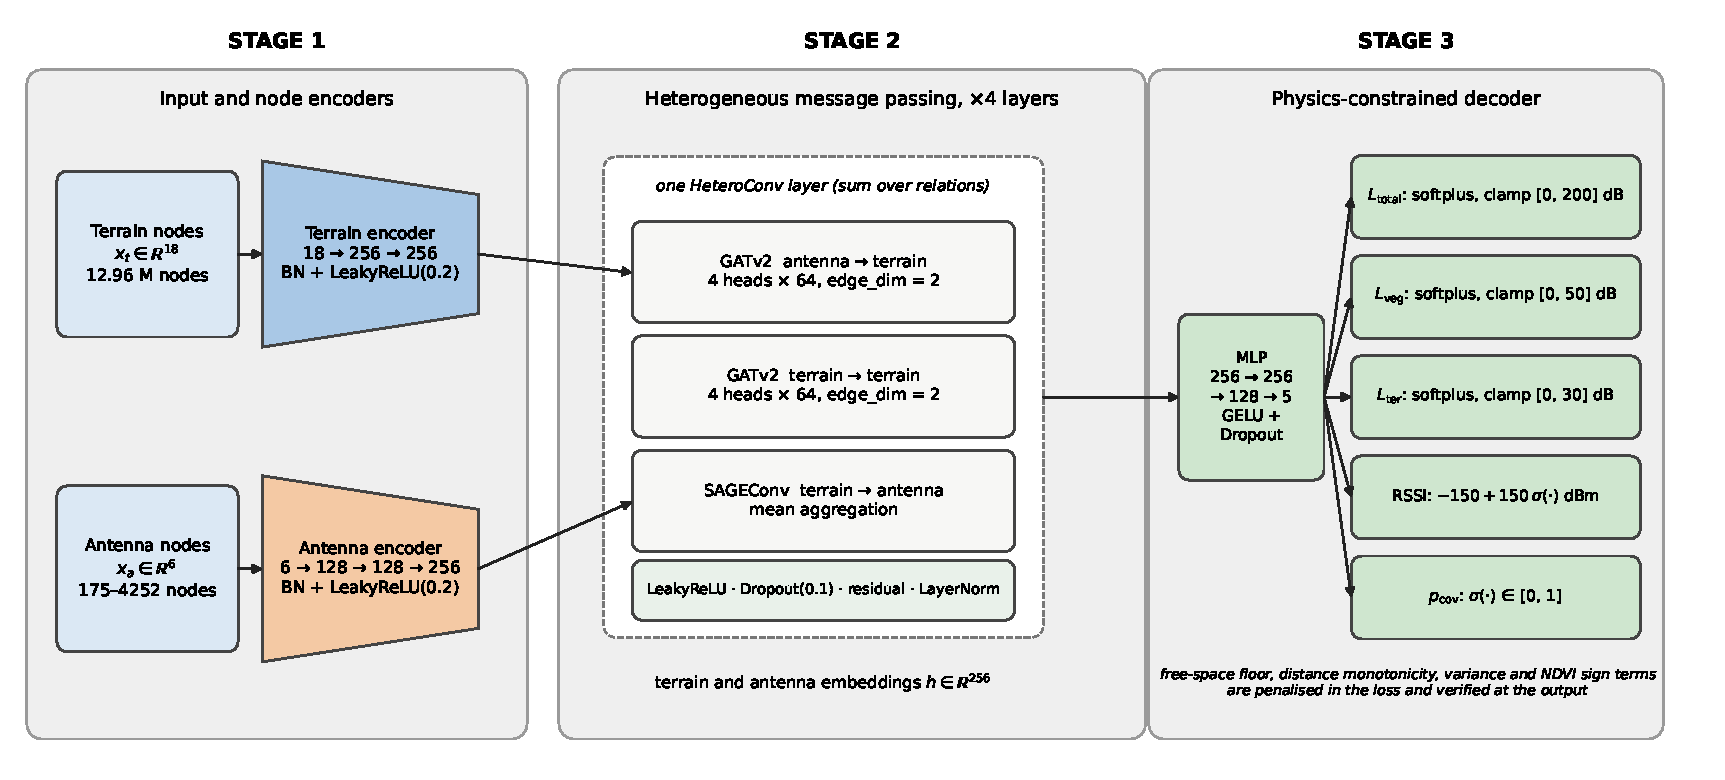
\includegraphics[width=0.95\textwidth]{novas/fig_arquitetura.pdf}
\caption{GNN-RF encoder--decoder architecture: type-specific terrain and antenna encoders, four heterogeneous GATv2 layers with residual connections, and a physics-constrained decoder with five RF outputs (hyperparameters in Table~\ref{tab:model_config}).}
\label{fig:architecture}
\end{figure*}

\subsubsection{Terrain encoder}

The terrain encoder (Fig.~\ref{fig:architecture}) maps raw features $\mathbf{x}_i^t \in \mathbb{R}^{18}$ to hidden representations:
\begin{equation}
\mathbf{h}_i^{t,(0)} = f_{\text{BN}}\!\bigl(\mathbf{W}_2^t \cdot \sigma(\mathrm{BN}(\mathbf{W}_1^t \mathbf{x}_i^t + \mathbf{b}_1^t)) + \mathbf{b}_2^t\bigr)
\label{eq:terrain_enc}
\end{equation}
where $\mathbf{W}_1^t \in \mathbb{R}^{d_h \times d_t}$, $\mathbf{W}_2^t \in \mathbb{R}^{d_h \times d_h}$, $\mathrm{BN}$ denotes batch normalization, $\sigma = \mathrm{LeakyReLU}(0.2)$, and dropout with rate 0.1 is applied after the first activation~\cite{srivastava2014dropout}.

\subsubsection{Antenna encoder}

The antenna encoder maps $\mathbf{x}_j^a \in \mathbb{R}^{6}$ through a three-layer MLP:
\begin{equation}
\begin{split}
\mathbf{h}_j^{a,(0)} ={}& f_{\text{BN}}\!\bigl(\mathbf{W}_3^a \cdot \sigma(\mathbf{W}_2^a \cdot \sigma(\mathrm{BN}(\mathbf{W}_1^a \mathbf{x}_j^a + \mathbf{b}_1^a)) + \mathbf{b}_2^a) \\
&+ \mathbf{b}_3^a\bigr)
\end{split}
\label{eq:antenna_enc}
\end{equation}
with intermediate dimension 128 and output $\mathbf{h}_j^{a,(0)} \in \mathbb{R}^{d_h}$.

\subsubsection{Heterogeneous GATv2 layers}

The encoder stacks $L{=}4$ heterogeneous convolutional layers, each a \texttt{HeteroConv} module that routes a distinct convolution to every relation. The two forward relations, \texttt{propagates\_to} and \texttt{connects\_to}, use GATv2Conv~\cite{brody2022attentive} with $K{=}4$ heads and per-head dimension $d_h/K{=}64$, consuming the 2D edge attributes so that attention can weight neighbors by geometry. The reverse relation \texttt{in\_range\_of} (terrain$\to$antenna) uses the cheaper SAGEConv with mean aggregation~\cite{hamilton2017inductive}, since antenna states are never decoded into predictions and the relation carries as many edges as the forward antenna-to-terrain relation (up to \num{10503392} per quadrant, Table~\ref{tab:graph_census}). Under the one-hop neighbor sampler used for training and inference, however, the reverse relation has no edges in any batch.

Each layer applies LeakyReLU activation, dropout with rate 0.1, residual connections (when dimensions match)~\cite{he2016deep}, and per-type LayerNorm:
\begin{equation}
\mathbf{h}_i^{(\ell)} = \mathrm{LN}\!\Bigl(\mathrm{Drop}\!\bigl(\sigma\bigl(\mathrm{HetConv}^{(\ell)}(\mathbf{h}^{(\ell-1)})\bigr)\bigr) + \mathbf{h}_i^{(\ell-1)}\Bigr)
\label{eq:gnn_layer}
\end{equation}

\subsubsection{Physics-constrained decoder}

The decoder maps terrain embeddings $\mathbf{h}_i^{(L)} \in \mathbb{R}^{d_h}$ to five predictions through an MLP with GELU activations:
\begin{equation}
\hat{\mathbf{y}}_i = \mathbf{W}_3^d \cdot \mathrm{GELU}(\mathbf{W}_2^d \cdot \mathrm{GELU}(\mathbf{W}_1^d \mathbf{h}_i^{(L)}))
\label{eq:decoder}
\end{equation}
with dimensions $d_h \to d_h \to d_h/2 \to 5$ and dropout with rate 0.1 after each GELU.

Physics constraints are enforced via output activation functions:
\begin{align}
\hat{L}_{\text{total}} &= \min\!\bigl(\mathrm{softplus}(\hat{y}_0),\; 200\bigr) \label{eq:constraint_pl} \\
\hat{L}_{\text{veg}} &= \min\!\bigl(\mathrm{softplus}(\hat{y}_1),\; 50\bigr) \\
\hat{L}_{\text{ter}} &= \min\!\bigl(\mathrm{softplus}(\hat{y}_2),\; 30\bigr) \\
\widehat{\text{RSSI}} &= -150 + 150 \cdot \sigma(\hat{y}_3) \quad \in [-150, 0]\;\text{dBm} \\
\hat{p}_{\text{cov}} &= \sigma(\hat{y}_4) \quad \in [0, 1] \label{eq:constraint_cov}
\end{align}
where $\mathrm{softplus}(x) = \ln(1 + e^x)$ ensures non-negative path loss and $\sigma$ denotes the sigmoid function.

\begin{table}[!t]
\centering
\caption{GNN-RF architectural hyperparameters. Antenna input: carrier frequency, transmit power, height, gain, latitude, longitude.}
\label{tab:model_config}
\begin{tabular}{lr}
\toprule
Parameter & Value \\
\midrule
Hidden dimension ($d_h$) & 256 \\
Number of GNN layers ($L$) & 4 \\
Attention heads ($K$) & 4 \\
Edge feature dimension & 2 \\
Output dimension & 5 \\
Dropout rate & 0.1 \\
Terrain input dimension ($d_t$) & 18 (17 informative) \\
Antenna input dimension ($d_a$) & 6 \\
Neighbor fan-out (antenna / terrain) & 20 / 8 \\
Training batch (seed nodes) & \num{24576} \\
Total parameters & \num{1812515} \\
\bottomrule
\end{tabular}
\end{table}

\subsection{Physics-informed loss function}
\label{sec:loss_function}

The composite loss function combines data-driven regression with four physics-informed regularization terms. All five output channels and all four regularizers are active from the first epoch, with no training phases.

\subsubsection{Prediction loss}

The primary loss uses Huber regression~\cite{huber1964robust} with $\delta{=}5.0$ and channel weights:
\begin{equation}
\begin{aligned}
\mathcal{L}_{\text{pred}} &= \sum_{c=0}^{4} w_c \cdot \mathcal{L}_{\text{Huber}}(\hat{y}_c, y_c; \delta{=}5.0).
\end{aligned}
\label{eq:loss_pred}
\end{equation}
In the training script used for every reported run the channel weights stay uniform ($w_c = 0.2$) and all five channels are active in every epoch.

\subsubsection{FSPL lower-bound constraint}

Total path loss must not fall below the theoretical free-space minimum (Eq.~\ref{eq:fspl}):
\begin{equation}
\mathcal{L}_{\text{FSPL}} = \frac{1}{N} \sum_{i=1}^{N} \mathrm{ReLU}\!\bigl(L_{\text{FSPL},i} - \hat{L}_{\text{total},i}\bigr)
\label{eq:loss_fspl}
\end{equation}
This term penalizes violations in the loss; unlike the bounds of Eqs.~(\ref{eq:constraint_pl})--(\ref{eq:constraint_cov}), it is not imposed by the output activation, and admissibility is verified on the predictions in Section~\ref{sec:physics_consistency}.

\subsubsection{Distance--attenuation monotonicity}

RF attenuation generally increases with distance from the transmitter. We encourage this prior as a soft regularizer by sampling $K{=}512$ random node pairs $(i,j)$ where $d_i < d_j$:
\begin{equation}
\mathcal{L}_{\text{dist}} = \frac{1}{|\mathcal{P}|} \sum_{(i,j) \in \mathcal{P}} \mathrm{ReLU}\!\bigl(\widehat{\text{RSSI}}_j - \widehat{\text{RSSI}}_i + 1\bigr)
\label{eq:loss_dist}
\end{equation}
where $\mathcal{P} = \{(i,j) : d_{\text{ant},i} < d_{\text{ant},j}\}$. The 1\,dB margin imposes a minimum decrease of RSSI from the node closer to the nearest antenna to the farther one, and the term is zero only when that decrease is reached. Because the reference field takes the maximum received level over all transmitters, the relation to the nearest antenna holds only on average, and the term is a regularizer rather than a property of the field.

\subsubsection{Variance preservation}

Predicted RSSI should preserve the spatial variance of the target distribution:
\begin{equation}
\mathcal{L}_{\text{var}} = \bigl[\mathrm{ReLU}(\sigma_{y_3} - \sigma_{\hat{y}_3})\bigr]^2
\label{eq:loss_var}
\end{equation}

\subsubsection{Vegetation--NDVI sign consistency}

Predicted vegetation attenuation should correlate positively with observed vegetation density:
\begin{equation}
\mathcal{L}_{\text{NDVI}} = \mathrm{ReLU}\!\bigl(0.15 - \rho(\hat{L}_{\text{veg}}, \text{NDVI})\bigr)
\label{eq:loss_ndvi}
\end{equation}
where $\rho$ denotes Pearson correlation and 0.15 is a minimum-correlation threshold. The term penalizes only a wrong-signed or negligible relation between predicted vegetation attenuation and NDVI, a sign condition motivated by, but not equivalent to, the vegetation attenuation model of \mbox{ITU-R} P.833~\cite{itu833}.

\subsubsection{Total loss}

The complete loss is:
\begin{equation}
\label{eq:loss_total}
\begin{split}
\mathcal{L} ={}& \sum_{c=0}^{4} w_c \mathcal{L}_{\text{Huber}}^{(c)} + \lambda_F \mathcal{L}_{\text{FSPL}} + \lambda_V \mathcal{L}_{\text{veg}} \\
&+ \lambda_d \mathcal{L}_{\text{dist}} + \lambda_v \mathcal{L}_{\text{var}} + \lambda_n \mathcal{L}_{\text{NDVI}}
\end{split}
\end{equation}
where $(\lambda_F, \lambda_V, \lambda_d, \lambda_v, \lambda_n) = (0.05, 0.1, 0.05, 0.02, 0.03)$. The vegetation term $\mathcal{L}_{\text{veg}}$ is a Huber penalty between $\hat{L}_{\text{veg}}$ and a simplified \mbox{ITU-R} P.833 attenuation computed from canopy height; no canopy-height layer is available in this study, so this term is inactive in every reported run, and the vegetation and terrain-diffraction channels are supervised only through their Huber terms in Eq.~(\ref{eq:loss_pred}) against the corresponding components of the reference generator, documented in the Supplementary Material.

\subsection{Sequential transfer learning protocol}
\label{sec:transfer}

Training follows a sequential transfer protocol across four geographic quadrants per city (Algorithm~\ref{alg:transfer}). Q1 trains from random initialization for 35~epochs at learning rate $10^{-3}$; subsequent quadrants fine-tune~\cite{jaiswal2026data} from the preceding best checkpoint for 20~epochs at $2 \times 10^{-4}$, resetting the optimizer and scheduler state. The cosine schedule decays to $\eta_{\min}{=}10^{-6}$, and float16 mixed precision uses a GradScaler. Section~\ref{sec:model_comparison} compares this schedule with training every quadrant from scratch.

\begin{algorithm}[!t]
\caption{Sequential Transfer Learning Protocol}
\label{alg:transfer}
\begin{algorithmic}[1]
\REQUIRE City $c$, seed $s$, quadrant graphs $\{G_{Q_1}, \ldots, G_{Q_4}\}$
\STATE Initialize model $\theta \sim \mathcal{N}(0, \text{fan-in}^{-1})$
\FOR{$q \in \{Q_1, Q_2, Q_3, Q_4\}$}
    \IF{$q = Q_1$}
        \STATE $\eta \gets 10^{-3}$; $E \gets 35$
    \ELSE
        \STATE $\theta \gets \theta^*_{q-1}$ \COMMENT{load best checkpoint}
        \STATE $\eta \gets 2 \times 10^{-4}$; $E \gets 20$
    \ENDIF
    \STATE optimizer $\gets$ AdamW$(\theta, \eta, \lambda_{\text{wd}}{=}10^{-5})$
    \STATE scheduler $\gets$ CosineWarmRestarts$(T_0{=}10, T_{\text{mult}}{=}2)$
    \FOR{epoch $= 1$ \TO $E$}
        \STATE Train with NeighborLoader (batch size $= 24{,}576$)
        \STATE Compute $\mathcal{L}$ (Eq.~\ref{eq:loss_total}) under AMP (float16)
        \STATE $\nabla\theta \gets$ clip$(\nabla\theta, \|\cdot\|_{\max}{=}0.5)$
        \STATE Update $\theta$; step scheduler
    \ENDFOR
    \STATE $\theta^*_q \gets \arg\min_{\text{epoch}} \text{MAE}_{\text{val}}$
\ENDFOR
\RETURN $\{\theta^*_{Q_1}, \ldots, \theta^*_{Q_4}\}$
\end{algorithmic}
\end{algorithm}


%% ====================================================================
\section{Experimental Methodology}
\label{sec:methodology}
%% ====================================================================

\subsection{Study area and datasets}

Experiments cover four cities in S\~{a}o Paulo state, Brazil: Bauru, Campinas, Lins, and Sorocaba, representing diverse urban morphologies from compact urban cores (Campinas) to mixed rural--urban landscapes (Lins). Each city is partitioned into four geographic quadrants (Q1--Q4), yielding 16 city--quadrant evaluation units. Transmitter parameters, with carrier frequencies of 778--3550~MHz and transmit powers of 33.0--53.0~dBm, come from the ANATEL licensing extract documented in the Supplementary Material. The generator reads only frequency, transmit power, antenna height, gain, and site coordinates from this extract and applies gain as a scalar in every direction. Azimuth, mechanical and electrical downtilt, half-power beamwidth, front-to-back ratio, and polarization are present in the same records but never consumed. Every physical tower therefore collapses into a stack of co-located omnidirectional sources that differ only in frequency, power, gain, and height, averaging 13.5 transmitters per tower in Lins and up to 49 in Campinas.

Every accuracy, control, and uncertainty result in this work is obtained under a spatially blocked partition~\cite{roberts2017cross}. Each quadrant graph is tiled into 10\,km blocks separated by a 2\,km exclusion buffer and assigned 70/15/15 by block to training, validation, and test with a fixed partition seed (42). Each partition is a graph of its own, holding only its terrain nodes and copies of all antenna nodes, so that no training terrain node is reachable from validation or test terrain through an antenna. The neighbor sampler draws one hop from terrain seed nodes, so no batch contains terrain-to-antenna edges, and each antenna state depends only on the antenna's own attributes.

Each cell holds 132 blocks (92 training, 20 validation, 20 test); the buffer, which trims validation and test only, discards 14.7--14.8\% of the tile nodes and leaves \num{817601} to \num{833593} test nodes per cell (Fig.~\ref{fig:partition}). The checkpoint of each run is selected on validation alone, and the test partition is scored once. All 16 cells are trained with five seeds (42--46), for 80~runs. Results quoted from the preliminary experiment, which used a random 90/10 node partition, are identified as such where they appear.

\begin{figure*}[!t]
\centering
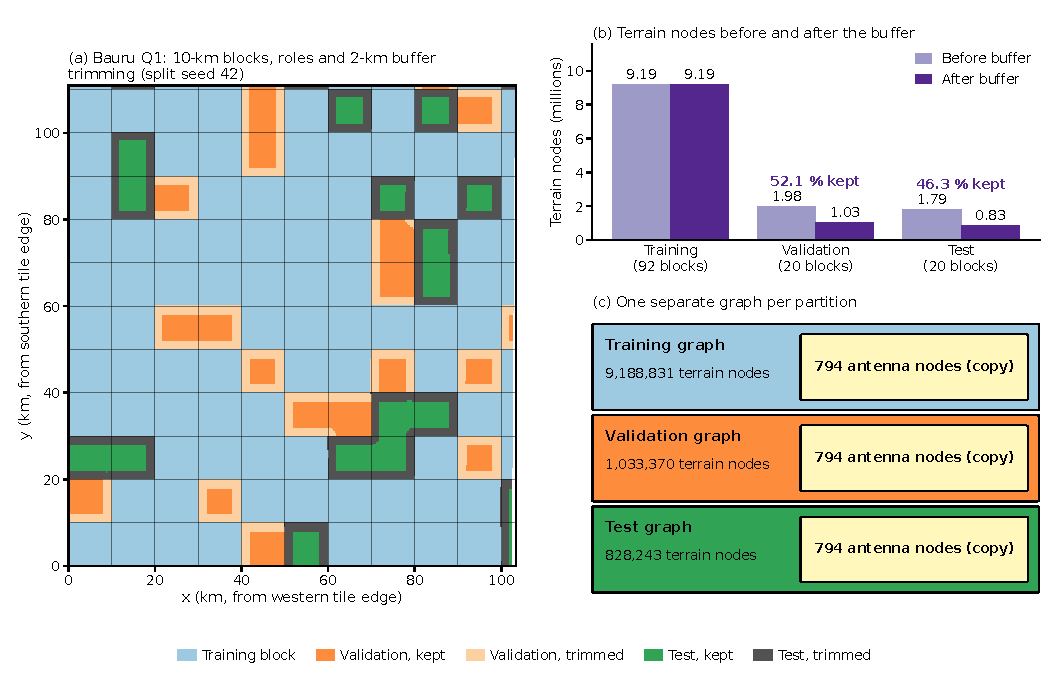
\includegraphics[width=\textwidth]{novas/fig_partition_R4min.pdf}
\caption{Spatially blocked partition, Bauru Q1. (a) 132 blocks of 10~km (92 training, 20 validation, 20 test; split seed 42) trimmed by a 2-km buffer. (b) Terrain nodes before and after the buffer. (c) Each partition is its own graph with a copy of all 794 antenna nodes, so no training terrain node is reachable from validation or test.}
\label{fig:partition}
\end{figure*}


The reference fields are produced by a deterministic propagation generator written for this study and documented equation by equation in the Supplementary Material: an Okumura--Hata base loss~\cite{hata1980empirical} up to 1500~MHz and COST\,231~\cite{cost231} above, a vegetation term driven by the node's NDVI, a terrain term driven by the node's slope, a two-term link budget, a best-server rule over all transmitters, a $-$110~dBm sentinel for unreached nodes, and coverage defined as RSSI above $-$85~dBm. The generator is point-local and traces no terrain profile between antenna and node. Recomputing the released total path loss from the features stored in the same files reproduces it with a mean absolute error of at most $3.02 \times 10^{-4}$\,dB per cell over \num{150000} valid-target nodes from five cells in the four cities, and every error reported in this paper measures fidelity to this generator.

Environment class is assigned once per transmitter from carrier frequency alone, not from a land-cover layer: urban above 1800~MHz, suburban between 800 and 1800~MHz, rural at or below 800~MHz. The best-server rule then searches every transmitter within a 30\,km inclusion radius and assigns each node to whichever one maximizes the received level, with no handover hysteresis or load-balancing offset, so the label describes the transmitter's band, not the ground beneath the node. Under these rules, of the \num{13186118} blocked test nodes of the 16 cells, \num{2247437} (17.04\%) are valid-target nodes, whose target path loss is valid rather than a sentinel value, and \num{182202} (1.38\% of test nodes, 8.11\% of valid-target nodes) have a target RSSI $\geq -85$~dBm, the coverage threshold.

The two auxiliary channels, vegetation attenuation and terrain diffraction, are computed in a later step than total path loss and RSSI, and the terrain term was corrected after generation. An early version of the generator filled each node's slope by an independent draw from a uniform distribution between 0.02 and 0.15 rather than reading the DEM; a corrector later replaced that draw with the node's actual DEM slope and recomputed total loss and RSSI by exact difference. Every field used in this paper's spatially blocked evaluation carries the corrected slope, while results quoted from the preliminary experiment predate the correction and use the uncorrected fields.

\subsection{Classical baselines}

Three analytical models serve as lower-bound references: FSPL (Eq.~\ref{eq:fspl}), Okumura--Hata Rural, that is, the open-area case of~\cite{hata1980empirical}, and COST\,231 Suburban~\cite{cost231}. Each is computed from the antenna parameters, distances, and frequencies of the graph data, calibrated on the training blocks of each cell only, and scored in absolute decibels on the same test nodes as GNN-RF, with the $-$110~dBm floor applied. Okumura--Hata and COST\,231 are kept as references even where the carrier lies outside their nominal bands~\cite{hata1980empirical,cost231}.

Each of the three models is evaluated under three calibration variants: (i)~a single 900~MHz reference frequency with the offset set to the training median, (ii)~the same reference with predicted RSSI clamped to the $-$110~dBm floor and the offset fitted on the clamped error, and (iii)~clamped with the per-link carrier frequency replacing the single 900~MHz reference, yielding nine calibrated candidates per cell. At a fixed frequency the Hata Rural and COST\,231 Suburban formulas differ by a constant that the calibrated offset absorbs, so their calibrated predictions coincide under variants (i) and (ii) and diverge only under variant~(iii).

\subsection{Learned baseline: an in-house RadioUNet-style adaptation}

The learned baseline, hereafter the node-wise adaptation, is an in-house encoder--decoder that carries the U-Net-style skip connections of RadioUNet~\cite{levie2021radiounet} into a fully connected network applied to each terrain node, with widths of 256, 128, and 64 and without convolution, raster, or terrain-to-terrain step. It shares the physics-constrained decoder and the loss of GNN-RF. Each terrain node supplies 44 inputs ($18 + 5 \times 5 + 1$): the 18 terrain inputs of GNN-RF; for each of up to five antenna-to-terrain links, ordered by increasing distance, the link distance and carrier frequency carried by the antenna-to-terrain edges of the graph, the effective isotropic radiated power (EIRP) of the transmitter, the antenna height, and a presence flag; and $\log(1+n)$ for $n$ links. The baseline consumes the antenna-to-terrain relations of the graph but receives neither the antenna coordinates nor any terrain-to-terrain relation.

With \num{369827} trainable parameters, about one fifth of the \num{1812515} of GNN-RF, the baseline is trained in 80 runs (four cities, four quadrants, seeds 42--46) with its own transfer chain. It shares the blocked split, the test nodes, the checkpoint rule, and the epoch budget of the GNN-RF reference runs, and it takes their optimization settings without a hyperparameter search. Each baseline run is paired with the reference run of the same city, quadrant, and seed.

\subsection{Ablation design}
\label{sec:ablation_design}

The ablation asks whether the relations of the graph, rather than parameter capacity, carry the accuracy of GNN-RF, by comparing it with the graph-free control, which receives no graph relation, and with the node-wise adaptation, which receives the antenna-to-terrain relations without message passing. The graph-free control replaces the architecture with a multilayer perceptron matched to GNN-RF in nominal parameters, holding exactly \num{1812515} trainable parameters and no antenna-to-terrain or terrain-to-terrain link, trained with the same loss, partition, checkpoint rule, and epoch budget on all four cities with five seeds each (16~cells, 80~paired runs). All of its parameters are active, whereas GNN-RF has \num{1484037} effective trainable parameters, a mismatch that favors the control and makes it conservative where GNN-RF has the lower error.

A second arm keeps the trained seed-42 models and damages the graph at test time on the eight cells of Lins and Bauru, with three shuffling seeds per arm: antenna-to-terrain edges are permuted preserving node degree, terrain-to-terrain edges are permuted the same way, both are permuted together, and message passing is removed by evaluating on an empty graph.

Two retrained arms test the objective: one (C1) sets the weights of all four penalty terms to zero, and the other (C2) sets only the monotonicity weight to zero, keeping the FSPL-floor, variance, and NDVI weights of the reference runs. Each arm has 80 runs with its own transfer chain, copies every other training setting from the corresponding reference run, and uses the same blocked split, test nodes, and evaluation, with its differences from the reference paired as for the learned baseline. The FSPL-floor penalty is essentially inactive in training, its weighted value never exceeding $6.06\times10^{-4}$ of the weighted RSSI data term in any epoch, so it has no retraining arm of its own.

\subsection{Evaluation metrics and statistical tests}
\label{sec:evaluation}

Primary metrics:
\begin{align}
\text{MAE} &= \frac{1}{N}\sum_{i=1}^{N} |\hat{y}_i - y_i| \label{eq:mae} \\
\text{RMSE} &= \sqrt{\frac{1}{N}\sum_{i=1}^{N} (\hat{y}_i - y_i)^2} \label{eq:rmse} \\
\text{P90} &= Q_{0.9}(|\hat{y}_i - y_i|) \label{eq:p90}
\end{align}

The unit of analysis for claims of geographic generalization is the city ($n{=}4$), with the cell ($n{=}16$, seeds as replicates) and the seed chain as secondary readings; terrain nodes are never the unit of a test, and the intraclass correlation of cell by seed is 0.73, so runs are not treated as independent either. Every results table names its node population (all test nodes or valid-target nodes) and reports the mean of cells unless stated as pooled; each run enters through its checkpoint of lowest validation RSSI MAE, and inference uses the neighbor-sampling evaluator with 20 antenna and 8 terrain neighbors per edge type.

Confidence intervals are computed over cells. Paired contrasts report the mean difference with a 95\% $t$ interval and the paired $t$ and Wilcoxon~\cite{wilcoxon1945individual,demsar2006statistical} $p$-values and, where absence of an effect is the question, two one-sided tests (TOST) at a \SI{0.1}{\deci\bel} margin fixed before the runs; comparisons among cities use Wilcoxon tests with Holm correction. Each seed enters through the mean of its cell, and where the city is the unit the interval is computed over the city means, without resampling at any level.

For the retrained arms and the learned baseline, each difference is the mean of 80 run-level differences paired by city, quadrant, and seed, with a 95\% interval from a hierarchical bootstrap ($B{=}\num{20000}$) that resamples cities and, within each city, seed chains with their four quadrants together. Differences are given as the arm or model minus GNN-RF, negative where the arm or model has the lower error. Such a difference is inconclusive relative to the pre-specified margin when its interval crosses that margin, fixed before the retrained and baseline runs at $\pm$\SI{0.045}{\deci\bel} for the MAE over all test nodes, $\pm$\SI{0.35}{\deci\bel} for the MAE over valid-target nodes, and $\pm$\SI{0.1}{\deci\bel} for the valid-target bias of the retrained arms. Each MAE margin is the minimum detectable effect at 80\% power of a paired two-sided $t$ test ($\alpha{=}0.05$, 16 city--quadrant cells) implied by the seed-to-seed variability of the 80 reference GNN-RF runs.

For uncertainty, prediction intervals are built at nominal levels $q \in \{50, 80, 90, 95, 99\%\}$ and scored by:
\begin{align}
\text{PICP}_q &= \frac{1}{N}\sum_{i=1}^{N} \mathbb{1}\!\bigl[y_i \in [\hat{y}_i^{\text{lo}}(q), \hat{y}_i^{\text{hi}}(q)]\bigr] \label{eq:picp} \\
\text{Width}_q &= \frac{1}{N}\sum_{i=1}^{N} \bigl(\hat{y}_i^{\text{hi}}(q) - \hat{y}_i^{\text{lo}}(q)\bigr) \label{eq:sharpness}
\end{align}
together with interval score, negative log-likelihood, and CRPS. The calibration region for split-conformal and deterministic-residual intervals is the validation blocks of the same cell, spatially separated from its test blocks, and a method is called calibrated only if $|\text{PICP}_q - q| \le 0.05$ at $q \in \{80, 90, 95\%\}$ in at least 12 of the 16 cells, a criterion fixed before the evaluation.

\subsection{Computational infrastructure}

All experiments ran on a workstation with a single NVIDIA RTX 5070 Ti GPU (16\,GB VRAM), using PyTorch 2.10 with CUDA 12.8 and PyTorch Geometric. Across the 80 blocked runs, peak training VRAM is 7430--7512~MB (median 7467~MB) and wall-clock time per run is 2181--4032~s (median 2292~s).


%% ====================================================================
\section{Results and Analysis}
\label{sec:results}
%% ====================================================================

\begin{table}[!t]
\centering
\caption{Results roadmap: MAE values and paired MAE differences of Section~\ref{sec:results}, all from the spatially blocked protocol with five seeds per cell except the empty-graph ablation, MC-mean, and cross-city rows (seed 42). Rows reading ``X minus GNN-RF'' give the paired difference in MAE, negative where X has the lower error; intervals and margins of the node-wise adaptation and of the retrained arms (C1, C2) follow Section~\ref{sec:evaluation}.}
\label{tab:results_roadmap}
\setlength{\tabcolsep}{3pt}
\begin{tabular}{@{}>{\raggedright\arraybackslash}p{3.3cm}lrl@{}}
\toprule
Context & Scope & MAE (dB) & 95\% CI (dB) \\
\midrule
Blocked test, all nodes & 16 cells & 0.395 & \\
Blocked test, valid-target nodes & 16 cells & 2.012 & \\
Node-wise adaptation minus GNN-RF, all nodes & 16 cells & $-$0.0571 & [$-$0.1183, $+$0.0025] \\
Node-wise adaptation minus GNN-RF, valid-target nodes & 16 cells & $-$0.7794 & [$-$1.8484, $-$0.1163] \\
Empty-graph ablation minus GNN-RF & 8 cells & $+$1.72 & \\
Graph-free control minus GNN-RF & 16 cells & $+$0.247 & \\
No-penalty retraining (C1) minus GNN-RF, all nodes & 16 cells & $-$0.0593 & [$-$0.1249, $+$0.0156] \\
No-penalty retraining (C1) minus GNN-RF, valid-target nodes & 16 cells & $+$0.1497 & [$-$0.3082, $+$0.8106] \\
No-monotonicity retraining (C2) minus GNN-RF, all nodes & 16 cells & $-$0.0865 & [$-$0.1323, $-$0.0391] \\
No-monotonicity retraining (C2) minus GNN-RF, valid-target nodes & 16 cells & $-$0.0768 & [$-$0.3512, $+$0.3093] \\
MC-mean, valid-target nodes & 16 cells & 2.35 & \\
Cross-city, full/zeroed topography & 3 cities & 0.40--3.93 & \\
\bottomrule
\end{tabular}
\end{table}

\subsection{Evaluation protocol and partition leakage}
\label{sec:eval_protocol}

A nearest-neighbor predictor exposes partition leakage on this reference field in all 16 cells. Restricting the copied training neighbor to a node with a valid target and sampling up to 20{,}000 valid-target test nodes per cell (seed 42), Table~\ref{tab:nn_contrast} reports its path-loss MAE under both partitions in every city--quadrant cell, with a median of 0.41\,dB under the random node split and 4.14\,dB under the spatially blocked split. The blocked-split MAE exceeds the random-split MAE in all 16 cells, with a median ratio of 10.5 (range 3.1--40.3) and a median gap of 3.80\,dB (range 1.52--6.45\,dB); the pre-specified presence criterion holds in all 16 cells and all four cities. A trivial copy of the nearest labeled neighbor is therefore adequate under random partitioning and fails under spatial blocking~\cite{ploton2020spatial}, so the partition rather than the predictor drives the gap.

\begin{table}[t]
\caption{Nearest-neighbour (1-NN) path-loss predictor under a random and a spatially blocked node partition, 16 city--quadrant cells (seed~42). The prediction for a test node is the path loss of the nearest training node with a valid path loss; MAE is computed on up to \num{20000} sampled test nodes with a valid path loss per cell. The random partition has the same training and test sizes as the blocked partition. Ratio is blocked over random MAE in each cell; summary rows give the median and range of each column. Cells share a seed and adjacent tiles, so medians and ranges are shown instead of confidence intervals.}
\label{tab:nn_contrast}
\centering
\small
\begin{tabular}{llccc}
\toprule
 & & \multicolumn{2}{c}{1-NN MAE (dB)} & \\
\cmidrule(lr){3-4}
City & Q & Random & Blocked & Ratio \\
\midrule
Bauru & Q1 & 0.39 & 6.65 & 17.2 \\
Bauru & Q2 & 0.26 & 4.23 & 16.2 \\
Bauru & Q3 & 0.49 & 2.01 & 4.1 \\
Bauru & Q4 & 0.39 & 4.12 & 10.5 \\
Campinas & Q1 & 0.35 & 4.76 & 13.6 \\
Campinas & Q2 & 0.87 & 2.89 & 3.3 \\
Campinas & Q3 & 0.55 & 4.17 & 7.6 \\
Campinas & Q4 & 0.99 & 4.92 & 4.9 \\
Lins & Q1 & 0.19 & 3.08 & 16.6 \\
Lins & Q2 & 0.16 & 6.61 & 40.3 \\
Lins & Q3 & 0.24 & 4.11 & 17.4 \\
Lins & Q4 & 0.21 & 2.18 & 10.4 \\
Sorocaba & Q1 & 0.44 & 5.10 & 11.7 \\
Sorocaba & Q2 & 0.87 & 2.73 & 3.1 \\
Sorocaba & Q3 & 0.77 & 7.03 & 9.2 \\
Sorocaba & Q4 & 1.08 & 4.05 & 3.7 \\
\midrule
Bauru & median & 0.39 & 4.17 & 13.4 \\
 & range & 0.26--0.49 & 2.01--6.65 & 4.1--17.2 \\
Campinas & median & 0.71 & 4.46 & 6.3 \\
 & range & 0.35--0.99 & 2.89--4.92 & 3.3--13.6 \\
Lins & median & 0.20 & 3.60 & 17.0 \\
 & range & 0.16--0.24 & 2.18--6.61 & 10.4--40.3 \\
Sorocaba & median & 0.82 & 4.57 & 6.5 \\
 & range & 0.44--1.08 & 2.73--7.03 & 3.1--11.7 \\
\midrule
All cells & median & 0.41 & 4.14 & 10.5 \\
 & range & 0.16--1.08 & 2.01--7.03 & 3.1--40.3 \\
\bottomrule
\end{tabular}
\end{table}


This contrast uses a single partition seed and a sample of up to 20{,}000 test nodes per cell, and its nearest-neighbor tie-break rule, inherited from the spatial index, was tested against an alternative rule in only three of the 16 cells (Bauru~Q3, Sorocaba~Q2, Lins~Q1) without a change in conclusion. The blocked test set holds 6.3--6.4\% of the tile after the buffer, and the two splits differ in the valid-target population of the test set.

In the preliminary experiment, label-shuffled controls raised RSSI MAE by factors of 3.29 to 10.35 in all 16 cells, whereas the geographic-split control, measured on a RadioUNet adaptation of that experiment, passed its own threshold in only 8 of 16 cells, failing in Q1 and Q3 of every city. That failure motivates the spatially blocked protocol of Section~\ref{sec:methodology} adopted throughout this paper.

\subsection{Model comparison and baselines}
\label{sec:model_comparison}

Under the spatially blocked protocol, GNN-RF is scored against empirical models calibrated on the training blocks and evaluated on the same test nodes (Tables~\ref{tab:results_roadmap} and~\ref{tab:blocked_three_pop}). Over all test nodes, mean RSSI MAE is \SI{0.395}{\deci\bel} (95\% CI [\num{0.309}, \num{0.480}], $n{=}16$ cells; [\num{0.304}, \num{0.485}] with the city as unit), ranging from \SI{0.215}{\deci\bel} in Lins~Q4 to \SI{0.812}{\deci\bel} in Campinas~Q3, whereas calibrated FSPL reaches 0.74--3.09\,dB and calibrated Hata Rural and COST\,231 Suburban 0.35--2.72\,dB on the same nodes. Over all test nodes, against the best calibrated empirical model of each cell, GNN-RF is more accurate in 15 of 16 cells and trails by \SI{0.009}{\deci\bel} in Campinas~Q2. Over the \num{2247437} valid-target nodes, GNN-RF reaches \SI{2.012}{\deci\bel} as the mean of cells and \SI{1.665}{\deci\bel} pooled by node (cells weighted by their valid-target nodes), against \SI{4.362}{\deci\bel} and \SI{4.935}{\deci\bel}, respectively, for the best calibrated empirical model of each cell on those nodes.

\begin{table*}[t]
\caption{Test error on the spatially blocked split, all 16 city--quadrant cells, three populations of test nodes: all nodes (sentinel included), nodes with a valid path-loss target (``valid-target''), and the valid-target subset for path loss. GNN-RF entries are mean $\pm$ s.d. over training seeds; MLP is the graph-free control of Section~\ref{sec:ablation_design} (all nodes; mean over training seeds). ``Best empirical'' is the lowest-error calibrated empirical model on the same nodes, chosen separately for the all-node and valid-target populations; ``Constant'' is the $-110$~dBm sentinel predictor. Every entry uses the checkpoint of lowest validation RSSI MAE and the test nodes of its population; each cell is the mean of five seeds, the last row is the unweighted mean of the 16 cells, and the evaluator is stochastic, sampling neighbors ($k_{\mathrm{antenna}}=20$, $k_{\mathrm{terrain}}=8$).}
\label{tab:blocked_three_pop}
\centering
\small
\resizebox{\textwidth}{!}{%
\begin{tabular}{ll c ccc c cc c c}
\toprule
 & & & \multicolumn{3}{c}{GNN-RF (dB)} & MLP & \multicolumn{2}{c}{Best empirical (dB)} & Constant & \\
City & Q & Valid-target frac. & RSSI, all & RSSI, valid-target & PL, valid-target & RSSI, all & RSSI, all & RSSI, valid-target & RSSI, all & seeds \\
\midrule
Bauru & Q1 & 0.328 & 0.632 $\pm$ 0.093 & 1.67 $\pm$ 0.34 & 2.21 $\pm$ 0.54 & 0.927 & 1.932 & 3.99 & 5.236 & 5 \\
Bauru & Q2 & 0.150 & 0.369 $\pm$ 0.073 & 1.62 $\pm$ 0.34 & 2.82 $\pm$ 0.65 & 0.373 & 0.982 & 4.33 & 1.694 & 5 \\
Bauru & Q3 & 0.159 & 0.391 $\pm$ 0.048 & 1.54 $\pm$ 0.30 & 2.14 $\pm$ 0.66 & 0.434 & 1.019 & 3.82 & 2.613 & 5 \\
Bauru & Q4 & 0.135 & 0.236 $\pm$ 0.071 & 1.09 $\pm$ 0.43 & 2.20 $\pm$ 1.10 & 0.205 & 0.806 & 3.61 & 2.077 & 5 \\
Campinas & Q1 & 0.241 & 0.495 $\pm$ 0.100 & 1.63 $\pm$ 0.45 & 3.76 $\pm$ 1.66 & 1.824 & 1.994 & 7.38 & 2.417 & 5 \\
Campinas & Q2 & 0.151 & 0.350 $\pm$ 0.205 & 1.71 $\pm$ 1.16 & 2.90 $\pm$ 3.00 & 0.315 & 0.341 & 1.30 & 2.636 & 5 \\
Campinas & Q3 & 0.297 & 0.812 $\pm$ 0.170 & 2.37 $\pm$ 0.54 & 3.55 $\pm$ 1.54 & 1.229 & 2.035 & 6.86 & 3.882 & 5 \\
Campinas & Q4 & 0.135 & 0.222 $\pm$ 0.078 & 1.12 $\pm$ 0.56 & 2.16 $\pm$ 1.51 & 0.568 & 0.787 & 2.98 & 2.087 & 5 \\
Lins & Q1 & 0.030 & 0.447 $\pm$ 0.072 & 9.65 $\pm$ 2.22 & 8.65 $\pm$ 2.35 & 0.366 & 1.200 & 3.69 & 1.130 & 5 \\
Lins & Q2 & 0.148 & 0.474 $\pm$ 0.065 & 2.64 $\pm$ 0.49 & 2.40 $\pm$ 0.59 & 0.172 & 0.484 & 1.65 & 4.334 & 5 \\
Lins & Q3 & 0.100 & 0.254 $\pm$ 0.049 & 0.95 $\pm$ 0.44 & 1.63 $\pm$ 0.64 & 0.227 & 0.436 & 3.02 & 1.830 & 5 \\
Lins & Q4 & 0.125 & 0.215 $\pm$ 0.040 & 1.04 $\pm$ 0.22 & 2.06 $\pm$ 0.75 & 0.230 & 0.802 & 2.94 & 1.927 & 5 \\
Sorocaba & Q1 & 0.221 & 0.379 $\pm$ 0.046 & 1.16 $\pm$ 0.25 & 2.16 $\pm$ 1.16 & 1.184 & 1.691 & 7.64 & 1.390 & 5 \\
Sorocaba & Q2 & 0.153 & 0.391 $\pm$ 0.120 & 1.84 $\pm$ 0.77 & 1.44 $\pm$ 0.82 & 0.264 & 0.401 & 1.12 & 2.428 & 5 \\
Sorocaba & Q3 & 0.220 & 0.419 $\pm$ 0.062 & 1.37 $\pm$ 0.27 & 3.21 $\pm$ 0.47 & 1.302 & 2.683 & 12.03 & 4.063 & 5 \\
Sorocaba & Q4 & 0.135 & 0.227 $\pm$ 0.035 & 0.82 $\pm$ 0.12 & 1.54 $\pm$ 0.50 & 0.656 & 0.652 & 3.44 & 1.665 & 5 \\
\midrule
\multicolumn{2}{l}{Mean of 16 cells} &  & 0.395 & 2.012 & 2.801 &  &  &  &  &  \\
\bottomrule
\end{tabular}%
}
\end{table*}


A paired test confirms this margin: against the best of nine calibrated analytical candidates in each cell, GNN-RF reduces mean RSSI MAE by \SI{0.746}{\deci\bel} (95\% CI [0.411, 1.080], $p{=}2.59\times10^{-4}$ paired $t$, $p{=}6.10\times10^{-5}$ Wilcoxon, Cohen's $d_z{=}1.19$). With the city as the unit ($n{=}4$), the margin is \SI{0.746}{\deci\bel} (95\% $t$ interval [0.331, 1.161], $p{=}0.0106$ paired $t$; Wilcoxon $p{=}0.125$, the minimum attainable with four cities), and GNN-RF is more accurate in all four cities. The 16 cells are not strictly independent, since quadrants of the same city are adjacent tiles, and selecting the best analytical candidate per cell is an optimistic envelope for the baseline, which is conservative for this claim.

On valid-target nodes, where the generator assigns a valid path loss, the margin widens: GNN-RF reaches 0.82--9.65\,dB RSSI MAE over all 16 cells, Lins~Q1 included, and 2.801\,dB path-loss MAE as the mean of cells, against 1.12--12.03\,dB for the best empirical model. It trails in four cells, Lins~Q1, where only 3\% of test nodes are valid-target (9.65 against 3.69\,dB), Lins~Q2 (2.64 against 1.65\,dB), Campinas~Q2 (1.71 against 1.30\,dB), and Sorocaba~Q2 (1.84 against 1.12\,dB). A constant $-$110~dBm predictor, scored on all test nodes, never comes within 0.5\,dB of GNN-RF in any of the 16 cells, so the all-node figure does not reduce to predicting the sentinel.

Table~\ref{tab:transfer_control} tests the sequential schedule of Section~\ref{sec:transfer} against training each non-head quadrant from scratch on the same blocked split. Over 24 pairs (four cities, seeds 42 and 43, Q2--Q4), the chained model differs from the from-scratch model by $-$0.014\,dB (95\% CI [$-$0.072, $+$0.045], $p{=}0.60$, eight city--seed clusters), and at this unit two one-sided tests exclude a difference larger than $\pm$0.1\,dB ($p{=}0.0051$). With the city as the unit of analysis ($n{=}4$, seeds and quadrants nested within cities), the chained-minus-scratch difference in RSSI MAE is $-$0.014\,dB (95\% CI [$-$0.107, $+$0.079], $t$ with 3 degrees of freedom). This interval crosses the pre-specified $\pm$0.1\,dB margin, so no systematic difference is detectable at the city unit (TOST $p{=}0.030$; minimum detectable difference at 80\% power, 0.12\,dB).

Two features of the chain qualify this comparison. Because the from-scratch runs use 35 epochs at $10^{-3}$ and the chained runs 20 epochs at $2\times10^{-4}$, the comparison detects no systematic advantage of chaining but does not give a clean estimate of its effect; a reversed chain Q4$\to$Q1 in Lins, on one seed, gives 0.392 against 0.399\,dB. The chain also brings the training blocks of one quadrant close to the test nodes of the next: in each Q2 cell, 10.97 to 11.07\% of the valid-target test nodes lie within 2\,km of the Q1 training blocks, and excluding them changes the valid-target RSSI MAE of GNN-RF by at most \SI{0.104}{\deci\bel}. Over all Q2--Q4 test nodes, the share within 2\,km of the training blocks of the previous quadrant is 1.11\% (\num{109745} of \num{9884081}), so this proximity moves the blocked error of GNN-RF only slightly.

\begin{table}[t]
\caption{Transfer chain versus training from scratch on the same blocked split (Section~\ref{sec:model_comparison}). Each pair compares the quadrant model obtained by fine-tuning from the previous quadrant (chained: 20 epochs, learning rate $2\times10^{-4}$) with a model trained from scratch on the same data and split (35 epochs, $10^{-3}$); test RSSI MAE in dB, all test nodes; $\Delta$ is chained minus scratch. The pairs form eight (city, seed) clusters ($n=8$) nested in the four cities ($n=4$).}
\label{tab:transfer_control}
\centering
\small
\setlength{\tabcolsep}{4pt}
\begin{tabular}{llcccc}
\toprule
City & Seed & Q & Scratch (dB) & Chained (dB) & $\Delta$ (dB) \\
\midrule
Bauru & 42 & Q2 & 0.316 & 0.470 & +0.154 \\
Bauru & 42 & Q3 & 0.417 & 0.373 & $-0.044$ \\
Bauru & 42 & Q4 & 0.364 & 0.248 & $-0.116$ \\
Bauru & 43 & Q2 & 0.272 & 0.315 & +0.044 \\
Bauru & 43 & Q3 & 0.411 & 0.419 & +0.008 \\
Bauru & 43 & Q4 & 0.351 & 0.353 & +0.002 \\
Campinas & 42 & Q2 & 0.348 & 0.267 & $-0.081$ \\
Campinas & 42 & Q3 & 0.850 & 0.648 & $-0.202$ \\
Campinas & 42 & Q4 & 0.194 & 0.185 & $-0.009$ \\
Campinas & 43 & Q2 & 0.332 & 0.241 & $-0.091$ \\
Campinas & 43 & Q3 & 0.974 & 0.870 & $-0.105$ \\
Campinas & 43 & Q4 & 0.291 & 0.189 & $-0.102$ \\
Lins & 42 & Q2 & 0.317 & 0.496 & +0.179 \\
Lins & 42 & Q3 & 0.212 & 0.337 & +0.125 \\
Lins & 42 & Q4 & 0.271 & 0.261 & $-0.010$ \\
Lins & 43 & Q2 & 0.496 & 0.449 & $-0.048$ \\
Lins & 43 & Q3 & 0.253 & 0.230 & $-0.024$ \\
Lins & 43 & Q4 & 0.179 & 0.168 & $-0.011$ \\
Sorocaba & 42 & Q2 & 0.484 & 0.593 & +0.109 \\
Sorocaba & 42 & Q3 & 0.468 & 0.505 & +0.038 \\
Sorocaba & 42 & Q4 & 0.238 & 0.258 & +0.020 \\
Sorocaba & 43 & Q2 & 0.365 & 0.360 & $-0.004$ \\
Sorocaba & 43 & Q3 & 0.468 & 0.431 & $-0.038$ \\
Sorocaba & 43 & Q4 & 0.289 & 0.170 & $-0.119$ \\
\bottomrule
\end{tabular}
\end{table}


The comparison between the node-wise adaptation and GNN-RF is inconclusive relative to the pre-specified margin in both primary populations. Over all test nodes, the RSSI MAE differs by \SI{-0.0571}{\deci\bel} (95\% CI [$-$0.1183, $+$0.0025], 80 paired runs; 0.3375 against 0.3946\,dB), an interval that crosses the margin of $\pm$\SI{0.045}{\deci\bel}. Over valid-target nodes, it differs by \SI{-0.7794}{\deci\bel} (95\% CI [$-$1.8484, $-$0.1163]; 1.2327 against 2.0122\,dB). This interval excludes zero on the side where the node-wise adaptation has the lower error but does not lie entirely beyond the margin of $-$0.35\,dB, so the difference is also inconclusive. The four city means of the valid-target difference are all negative (Bauru $-$0.3116, Campinas $-$0.2504, Lins $-$2.3295, and Sorocaba $-$0.2263\,dB). The largest in magnitude falls in Lins, whose test blocks differ in composition from those of the other cities.

The valid-target test nodes of Lins~Q1 and Q2 are dominated by nodes at or above the $-$85~dBm coverage threshold. Of the valid-target test nodes, 93.2\% in Lins~Q1 (\num{23249} of \num{24945}) and 89.2\% in Lins~Q2 (\num{109989} of \num{123306}) have a target RSSI of at least $-$85~dBm, against 0 to 12.0\% in the other 14 cells. On this population, over the seven cells with at least \num{1000} such nodes, the mean-of-cells RSSI MAE is 2.631\,dB for the node-wise adaptation against 7.931\,dB for GNN-RF, and the node-wise adaptation has the lower error in 34 of the 35 paired runs (Table~\ref{tab:cov85_ba1}).

\begin{table}[!t]
\centering
\caption{RSSI MAE of the node-wise adaptation and of GNN-RF on valid-target test nodes with target RSSI of at least $-$85\,dBm, in the seven cells with at least \num{1000} such nodes (each cell the mean of five seeds; 35 paired runs). Nodes: number of test nodes of this population in the cell. The mean of cells is computed before rounding. The node-wise adaptation has the lower error in every cell. The population is described per cell, without an interval or a test.}
\label{tab:cov85_ba1}
\setlength{\tabcolsep}{4pt}
\begin{tabular}{lrcc}
\toprule
Cell & Nodes & Node-wise adapt. & GNN-RF \\
 & & MAE (dB) & MAE (dB) \\
\midrule
Bauru~Q1 & \num{7801} & 4.466 & 12.010 \\
Bauru~Q3 & \num{1151} & 0.572 & 2.115 \\
Campinas~Q1 & \num{6268} & 4.907 & 15.351 \\
Campinas~Q3 & \num{29223} & 3.790 & 10.412 \\
Lins~Q1 & \num{23249} & 3.566 & 10.049 \\
Lins~Q2 & \num{109989} & 0.553 & 2.754 \\
Sorocaba~Q3 & \num{4505} & 0.562 & 2.823 \\
\midrule
Mean of cells & & 2.631 & 7.931 \\
\bottomrule
\end{tabular}
\end{table}


The remaining contrasts of the node-wise adaptation are descriptive and carry no pre-specified margin. Valid-target path loss differs from that of GNN-RF by \SI{-1.0312}{\deci\bel} (95\% CI [$-$1.9267, $-$0.1718]), whereas on sentinel nodes the RSSI MAE of the node-wise adaptation is the higher one, with a difference of \SI{+0.0162}{\deci\bel} (95\% CI [$+$0.0012, $+$0.0299]). Against the graph-free control, the node-wise adaptation has a lower RSSI MAE, with differences of \SI{-0.3046}{\deci\bel} over all test nodes (95\% CI [$-$0.5292, $-$0.0781]) and \SI{-1.5060}{\deci\bel} over valid-target nodes (95\% CI [$-$2.4580, $-$0.5542]). Both learners that receive the antenna-to-terrain relations of the graph, the node-wise adaptation and GNN-RF, thus have a lower error than the graph-free control. On valid-target nodes, the best calibrated empirical model of each cell (\SI{4.362}{\deci\bel}, Table~\ref{tab:blocked_three_pop}) trails both.

\subsection{Multi-target reconstruction and physics decomposition}
\label{sec:multitarget}

GNN-RF reconstructs the two operationally primary RF fields, total path loss and RSSI, directly in absolute decibels from a single multi-output head, with the valid-target errors given in Section~\ref{sec:model_comparison}, and the same decoder emits a coverage probability. Because coverage in the reference field is RSSI thresholded at $-$85~dBm, this output is a derived classification rather than an independent target.

The remaining two channels, vegetation attenuation and terrain diffraction, are supervised against the corresponding components of the generator, which are computed at a single 1800~MHz carrier and toward the nearest transmitter (documented in the Supplementary Material), and are reported as auxiliary outputs. Over valid-target nodes, GNN-RF reaches a mean-of-cells MAE of 1.11\,dB on the vegetation channel and 0.83\,dB on the diffraction channel. In the generator, the slope-based terrain term, local to each node, enters the total path loss, whereas the midpoint-obstacle knife-edge term, whose loss approximates the single knife-edge formulation of ITU-R P.526~\cite{itu526}, enters only the diffraction channel, computed toward the nearest transmitter.

The coverage class holds 1.38\% of test nodes and 8.11\% of valid-target nodes, and the probability output cut at 0.5 agrees with the predicted RSSI thresholded at $-$85~dBm on 99.61\% of test nodes, pooled over cells and seeds (Cohen's $\kappa{=}0.78$). Against the label defined by the target RSSI, the thresholded predicted RSSI reaches an F1 of 0.547 and the probability output, cut at the fixed value of 0.5, an F1 of 0.441, as the mean of the nine cells that contain both classes.

\subsection{Free-space-floor admissibility}
\label{sec:physics_consistency}

Free-space-floor admissibility is verified on the output rather than imposed: for each test node, the floor is set by the distance to the nearest transmitter at 1800\,MHz. Of the 80 blocked runs, 69 have no test node below the floor, and across all runs \num{2536} of \num{65930590} test nodes fall below it, unevenly distributed by city (Table~\ref{tab:physics_compliance}). This diagnostic is a bound test rather than the floor of the target: it takes the nearest transmitter at a fixed 1800\,MHz carrier, whereas the generator serves each node from the strongest transmitter at that link's carrier.

With the serving transmitter's distance and carrier, $1.39\times10^{-4}$ of valid-target test nodes fall below the free-space floor as the mean of cells ($1.10\times10^{-4}$ pooled), \num{1235} node-run violations out of \num{11237185} valid-target test-node evaluations, all from 9 of the 80 runs in four cells (Bauru~Q1, Campinas~Q1, Campinas~Q3, and Lins~Q1). A constant predictor, the median of the valid targets outside the test partition, never falls below the floor in any of the 16 cells (minimum margin 29.7\,dB), so passing the floor does not separate a physical field from a degenerate one. The NDVI term of Eq.~(\ref{eq:loss_ndvi}) is a sign condition on a correlation rather than a per-node relation, so no per-node vegetation fraction is reported.

\begin{table}[!t]
\centering
\caption{Free-space-floor admissibility of GNN-RF over the 80 blocked runs, all test nodes, with the floor at the distance to the nearest transmitter and 1800~MHz (Section~\ref{sec:physics_consistency}). Node counts are recovered from the recorded per-run fraction and number of test nodes. The last block repeats the test on the valid-target nodes with the distance and carrier of the transmitter that serves each node.}
\label{tab:physics_compliance}
\setlength{\tabcolsep}{4pt}
\begin{tabular}{lccc}
\toprule
City & Runs with no node & Nodes below & Test nodes \\
 & below the floor & the floor & evaluated \\
\midrule
Bauru & 18 of 20 & \num{115} & \num{16458440} \\
Campinas & 13 of 20 & \num{2118} & \num{16438370} \\
Lins & 18 of 20 & \num{303} & \num{16582940} \\
Sorocaba & 20 of 20 & \num{0} & \num{16450840} \\
\midrule
Total & 69 of 80 & \num{2536} & \num{65930590} \\
\midrule
\multicolumn{4}{l}{Serving transmitter, valid-target nodes} \\
Total & 71 of 80 & \num{1235} & \num{11237185} \\
\bottomrule
\end{tabular}
\end{table}





\subsection{Robustness and ablation}
\label{sec:robustness}

\begin{figure}[!t]
\centering
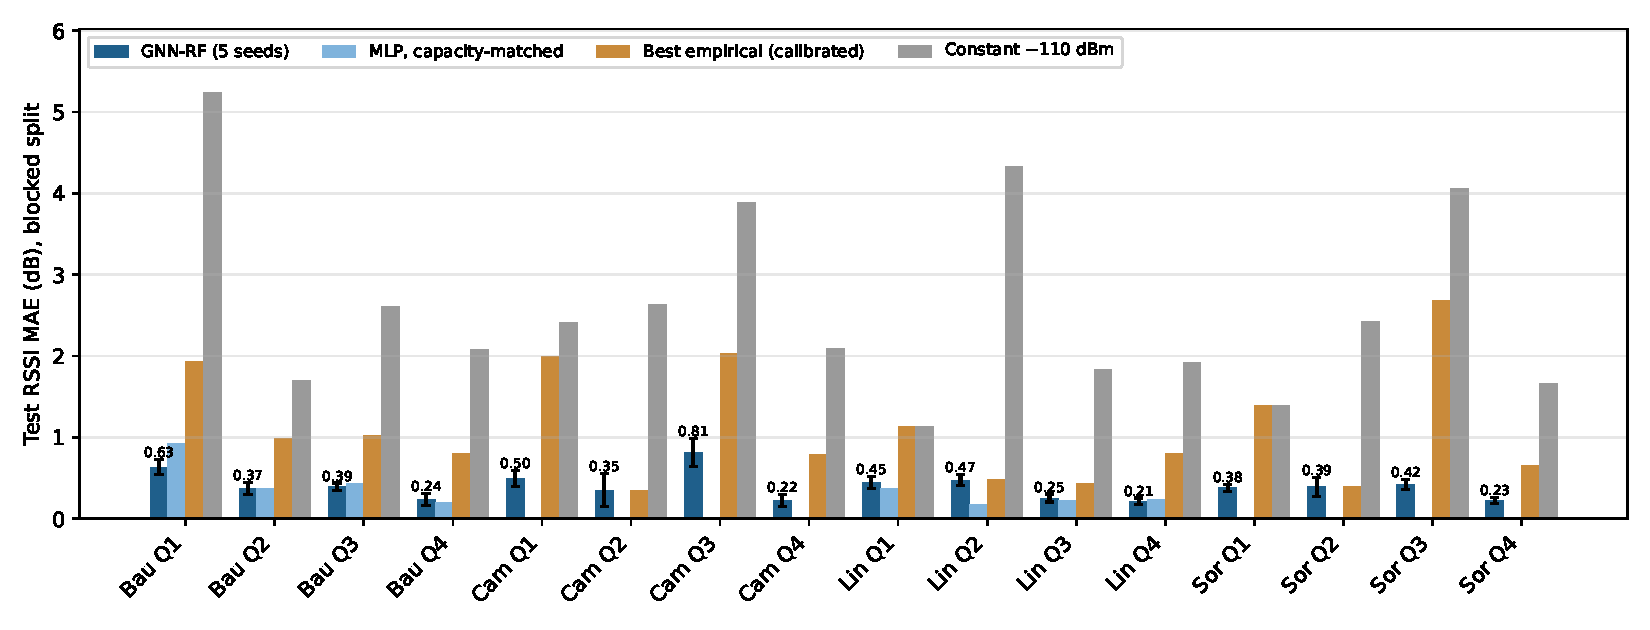
\includegraphics[width=\columnwidth]{novas/fig_blocked_16.pdf}
\caption{RSSI MAE on the spatially blocked test partition for all 16 city--quadrant cells (five training seeds each).}
\label{fig:multiseed}
\end{figure}

City means rise from 0.348\,dB in Lins through 0.354\,dB in Sorocaba and 0.407\,dB in Bauru to 0.470\,dB in Campinas, and across the 80 blocked runs variation between cells dominates variation between seeds (Section~\ref{sec:evaluation}; Fig.~\ref{fig:multiseed}). Against this variation, Table~\ref{tab:structural_ablation} and Fig.~\ref{fig:ablacao_estrutural} report how much test RSSI MAE degrades when the graph of a trained model is damaged, paired by cell over the eight Lins and Bauru cells. Shuffling antenna-to-terrain edges adds 0.18\,dB, shuffling terrain-to-terrain edges 0.67\,dB, shuffling both 0.80\,dB, and removing all edges 1.72\,dB. Terrain-to-terrain connectivity matters more than antenna-to-terrain connectivity in seven of the eight cells, the exception being Bauru~Q2, and in Lins~Q1 the empty graph barely changes the error (0.132\,dB). Only the direction of the difference between arms is reported, since eight cells leave their ratio too uncertain to quote.

The graph-free control (Section~\ref{sec:ablation_design}) covers all four cities rather than the two cities of the ablation above. At the city unit ($n{=}4$), the primary analysis, GNN-RF has lower mean RSSI MAE than the graph-free control by \SI{0.247}{\deci\bel}, but the 95\% CI crosses zero ($p{=}0.205$); with only four cities, no two-sided non-parametric test on this design can reach $p<0.125$, a bound that applies to any per-city result quoted from this control.

At the finer cell unit ($n{=}16$), the mean difference is unchanged and its significance is sensitive to the inferential method (95\% CI [$-$0.482, $-$0.013], $p{=}0.0397$ paired $t$, $p{=}0.117$ Wilcoxon); the same direction and magnitude hold at the chain unit ($n{=}20$, $p{=}0.00103$). The chain unit shares a Q1 checkpoint and spatial adjacency across its four cells, so it does not add an independent estimate of the effect beyond the cell-level reading above.

The sign of the advantage survives every leave-one-city-out window, but its size does not: excluding Campinas or Sorocaba roughly halves the mean effect (\num{-0.159} and \num{-0.164}\,dB, against \num{-0.363} excluding Lins and \num{-0.304} excluding Bauru). This pattern implies that Lins's own contribution to the aggregate runs opposite in sign to the other three cities. Across the 16 cells, the advantage correlates moderately with the fraction of valid-target test nodes ($r{=}-0.56$), an association that is exploratory and does not establish a causal relationship.

Retraining GNN-RF without any penalty term (C1) is inconclusive relative to the pre-specified margin in both primary populations. Over all test nodes the RSSI MAE differs by \SI{-0.0593}{\deci\bel} (95\% CI [$-$0.1249, $+$0.0156], 80 paired runs), and over valid-target nodes by \SI{+0.1497}{\deci\bel} (95\% CI [$-$0.3082, $+$0.8106]). Lins dominates the valid-target interval, with a city mean of $+$0.9916\,dB against $-$0.2669 to $-$0.0026\,dB in the other three cities. Without any penalty, the same architecture still keeps a mean error well below that of the best calibrated empirical model of each cell, 0.335 against 1.140\,dB over all test nodes and 2.162 against 4.362\,dB over valid-target nodes.

Removing only the monotonicity term (C2) is also inconclusive, although its all-node interval excludes zero. Over all test nodes the difference is \SI{-0.0865}{\deci\bel} (95\% CI [$-$0.1323, $-$0.0391]), an interval that crosses the margin of $-$0.045\,dB, and over valid-target nodes it is \SI{-0.0768}{\deci\bel} (95\% CI [$-$0.3512, $+$0.3093]). Sentinel nodes account for a fraction of 0.817 of the all-node difference, under an exact per-run decomposition of the all-node MAE into its valid-target and sentinel parts defined after the runs.

The bias of C2, the mean signed error of prediction minus target, is inconclusive on valid-target nodes against its margin of $\pm$0.1\,dB, set before the runs. There it changes by $+$0.1174\,dB for RSSI (95\% CI [$-$0.4070, $+$0.8791]) and by $-$0.4822\,dB for path loss (95\% CI [$-$1.4799, $+$0.7790]), and both intervals cross that margin. On sentinel nodes, where the same $\pm$0.1\,dB serves as a criterion set after the runs, the mean signed RSSI error shifts by $+$0.0245\,dB (95\% CI [$+$0.0049, $+$0.0412]) and stays inside it.

The physical admissibility of the outputs of C1 and C2 differs from that of the reference runs only within intervals that contain zero. Table~\ref{tab:admissibility_blocked} reports two quantities per model: the fraction of valid-target nodes predicted below the free-space floor of their serving transmitter, and the fraction of same-transmitter pairs in which the farther node is predicted more than 1\,dB stronger than the nearer one. For GNN-RF, the node-wise adaptation, and the graph-free control, none of the predicted floor violations falls on a node where the target itself lies below the floor.

\begin{table*}[t]
\caption{Structural ablation on the spatially blocked test split (all test nodes). The four edge-ablation rows use Lins and Bauru (Q1--Q4, seed~42 checkpoints; $n=8$ cells, three shuffling seeds per arm); entries are the change in test RSSI MAE relative to the trained model with the real graph, paired by cell; positive means worse. The last three rows are a different contrast: the paired difference GNN-RF minus the graph-free control (Section~\ref{sec:ablation_design}), in all four cities with five training seeds per cell, tested in the three pre-specified units (city; city--quadrant cell; seed chain, the mean of the four quadrants of one seed); negative means GNN-RF is more accurate. Cells and chains are not independent, since Q2--Q4 inherit the Q1 checkpoint of the same seed.}
\label{tab:structural_ablation}
\centering
\begin{tabular}{lccc c}
\toprule
Arm & $\Delta$MAE (dB) & 95\% CI & $p$ (paired $t$) & $p$ (Wilcoxon) \\
\midrule
Antenna$\to$terrain edges shuffled (degree preserved) & +0.181 & [+0.019; +0.343] & 0.0332 & 0.0391 \\
Terrain$\to$terrain edges shuffled (degree preserved) & +0.673 & [+0.262; +1.084] & 0.0061 & 0.0078 \\
Both relations shuffled & +0.798 & [+0.428; +1.169] & 0.0014 & 0.0078 \\
Empty graph (no message passing) & +1.723 & [+0.773; +2.674] & 0.0036 & 0.0078 \\
\midrule
\multicolumn{5}{l}{GNN-RF minus graph-free control (MLP, 1{,}812{,}515 nominal params), four cities} \\
\quad unit: city ($n=4$) & $-0.247$ & [$-0.736$; +0.241] & 0.2051 & 0.3750 \\
\quad unit: cell ($n=16$) & $-0.247$ & [$-0.482$; $-0.013$] & 0.0397 & 0.1167 \\
\quad unit: seed chain ($n=20$) & $-0.247$ & [$-0.381$; $-0.114$] & 0.0010 & 0.0032 \\
\bottomrule
\end{tabular}
\end{table*}


\begin{table}[!t]
\centering
\caption{Physical admissibility of the outputs under the blocked protocol, for the two quantities of Section~\ref{sec:robustness}. Floor: mean of 80 runs per model. Monotonicity: pairs of valid-target nodes whose distances to their shared serving transmitter differ by a factor of at least 2, mean of 40 runs per model over the 8 of 16 cells that have such pairs. The reference-field row scores the target itself (floor: mean of the 16 cells; monotonicity: mean of the 8 cells, with the maximum of a single cell in parentheses). The 95\% intervals of the paired differences of C1 and C2 against the reference contain zero for both quantities.}
\label{tab:admissibility_blocked}
\setlength{\tabcolsep}{3pt}
\begin{tabular}{@{}>{\raggedright\arraybackslash}p{3.4cm}>{\centering\arraybackslash}p{2.2cm}>{\centering\arraybackslash}p{2.2cm}@{}}
\toprule
Model & Below floor (fraction, 80 runs) & Monotonicity violations (fraction, 40 runs) \\
\midrule
GNN-RF (reference) & $1.39\times10^{-4}$ & 0.0446 \\
No-penalty retraining (C1) & $9.21\times10^{-5}$ & 0.0378 \\
No-monotonicity retraining (C2) & $1.14\times10^{-5}$ & 0.0304 \\
Node-wise adaptation & $2.04\times10^{-5}$ & 0.0017 \\
Graph-free control & 0 & 0.0252 \\
Reference field & $2.43\times10^{-4}$ & $4.14\times10^{-4}$ (0.0033) \\
\bottomrule
\end{tabular}
\end{table}


\begin{figure}[!t]
\centering
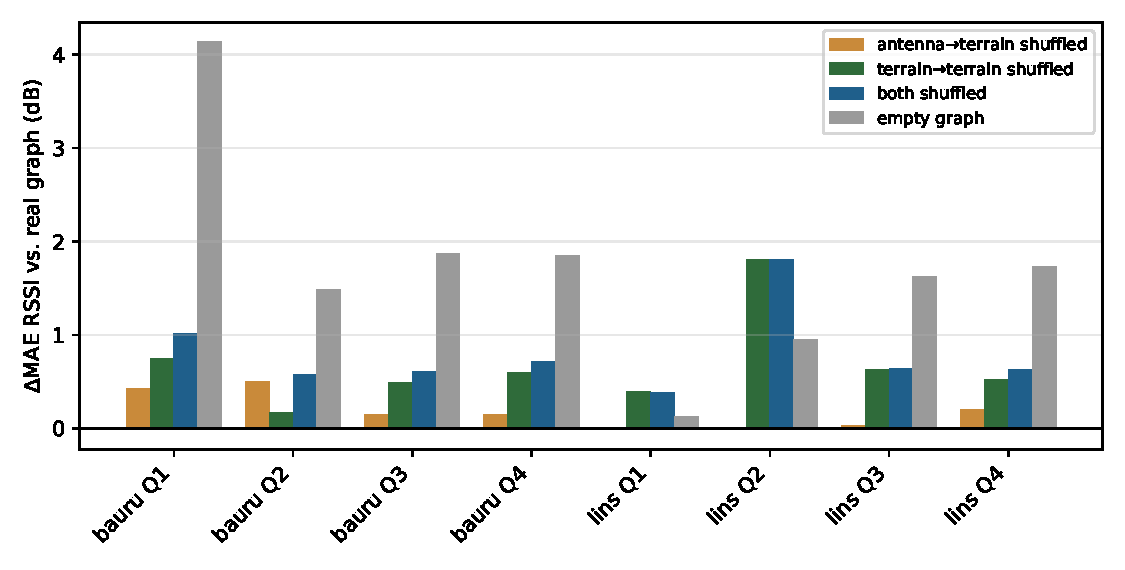
\includegraphics[width=\columnwidth]{novas/fig_ablacao_estrutural.pdf}
\caption{Structural ablation on the spatially blocked test split: change in RSSI MAE per cell from shuffling one edge relation, both relations, or removing all edges, relative to the trained model on the real graph (Lins and Bauru, Q1--Q4, seed-42 checkpoints).}
\label{fig:ablacao_estrutural}
\end{figure}

\subsection{Spatial error analysis}
\label{sec:spatial}

Test-set RSSI MAE decomposes very differently between the two populations that make up each cell. In all four cities, nodes with a valid path-loss target concentrate most of the absolute error, while sentinel nodes ($-$110\,dBm) carry near-zero MAE: valid-target MAE ranges from \SI{1.296}{\deci\bel} (Sorocaba) to \SI{3.571}{\deci\bel} (Lins) as city means over four cells and five seeds, against \SI{0.134}{\deci\bel} for the sentinel population as the mean of cells, and the valid-target population accounts for 71.89\% of total absolute error, pooled over cells and seeds.

The blocked split's geometry bounds how far a test node can be from training data. Across the four cities, no test node lies farther than \SI{8.58}{\kilo\meter} from the nearest training block edge, and the minimum distance falls between \num{1.963} and \SI{1.971}{\kilo\meter}, consistent with the pre-specified 2\,km exclusion buffer. Of the 20 test blocks the split lays out per city, only 17 (Bauru, Campinas, Lins) or 15 (Sorocaba) contain a node in the released dataset, because the last 10\,km grid strip covers only about \SI{0.97}{\kilo\meter} of the tile's extent; the rest of the nominal 20 blocks are geometrically empty, not missing data.

Error is spatially concentrated within the test area (Fig.~\ref{fig:spatial_error}, signed RSSI error of the seed-42 models on the Q1 test nodes of each city). Half of the total absolute RSSI error, all test nodes included, falls within a fraction of the tile that ranges from 1.5\% in Lins to 10.0\% in Sorocaba, wider (5.3\% to 27.5\%) for valid-target nodes. Comparing near-training ($<3$\,km) against far ($\geq5$\,km) valid-target MAE within the same test block, 8 of the 10 blocks large enough to pair (three in Bauru, four in Campinas, three in Sorocaba; Lins has none with enough valid-target nodes on both sides) show lower error near the training boundary, a border-optimism signal with a median paired ratio of 0.872. The city-pooled ratio inverts this signal in Bauru and Campinas, a Simpson's-paradox risk anticipated before the result, so the evidence used here is the paired-by-block reading, not the city pool.

The spatial correlation of the valid-target residual at short lag bins is well below that of the target field itself: at 1--2\,km it is 0.53 in Bauru and 0.58 in Lins, against 0.93 and 0.90 for the reference field at the same bin, indicating that most of the target's long-range structure is already explained rather than left in the residual. The formal range estimate saturates at the 50\,km grid ceiling in Bauru and Campinas, a sign of instability from few pairs at long distances, not of real structure, and is not reported as a single comparable range.

\begin{figure*}[!t]
\centering
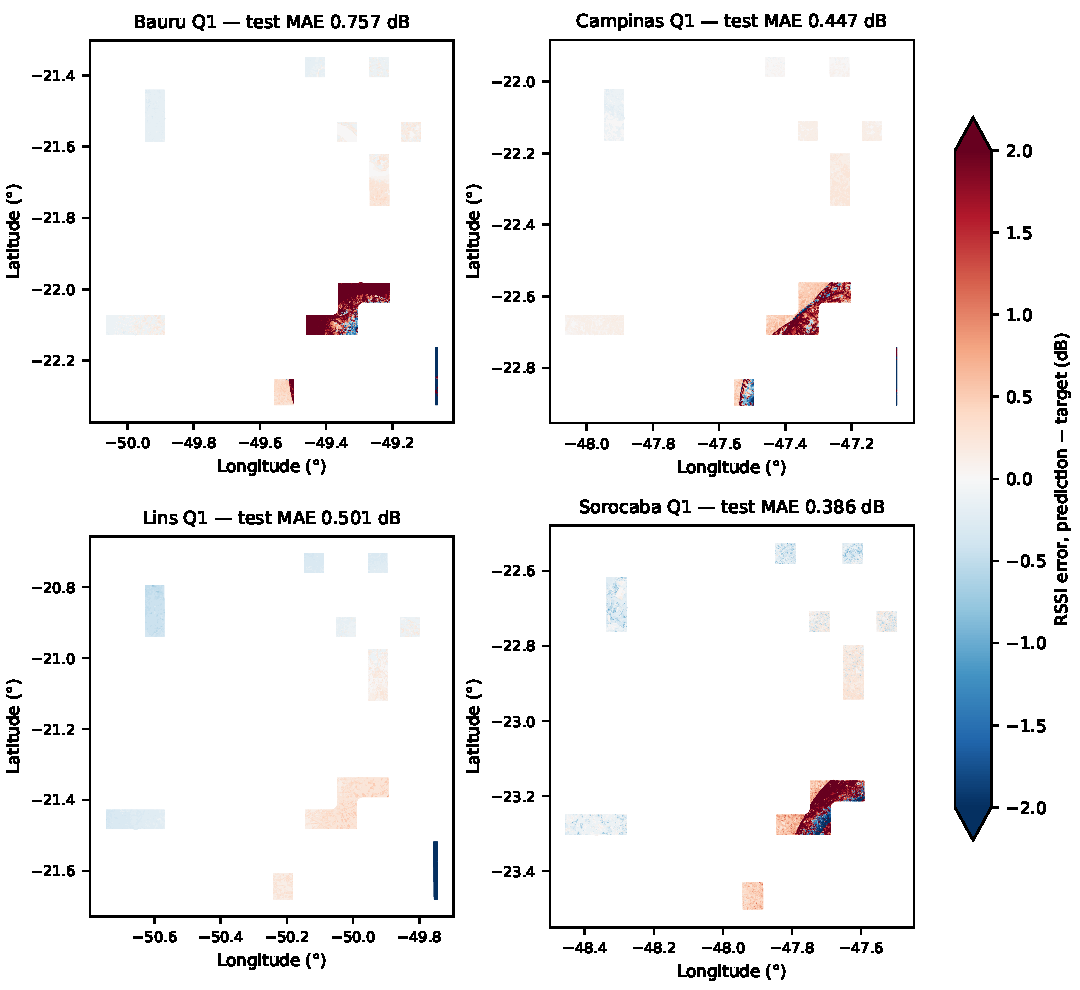
\includegraphics[width=0.8\textwidth]{novas/fig_erro_espacial_Q1.pdf}
\caption{Signed RSSI prediction error (prediction $-$ target, dB, color scale clipped at $\pm$2\,dB) on the spatially blocked test nodes of Q1 in each city (seed~42); the rectangles are the test blocks, whose layout repeats across cities because every partition uses the same block grid and seed. Axes in degrees of longitude and latitude.}
\label{fig:spatial_error}
\end{figure*}

\subsection{Uncertainty under spatially blocked evaluation}
\label{sec:uncertainty}

Epistemic dispersion is estimated by Monte Carlo Dropout~\cite{gal2016dropout} with $T{=}50$ stochastic passes on the 16 seed-42 checkpoints, activating only the dropout layers, attention dropout in the GATv2 layers included. Intervals come from the MC percentiles at five nominal levels, from a split-conformal correction calibrated on the validation blocks of each cell, and, as a baseline, from the validation residuals of the deterministic model (Table~\ref{tab:uncertainty_blocked}, Fig.~\ref{fig:calibracao_T14}). On valid-target test nodes, MC Dropout intervals contain the target in 0.369, 0.592, 0.683, 0.738, and 0.801 of cases at the 50, 80, 90, 95, and 99\% levels.

The conformal correction reaches 0.610 to 0.951 on average, but its 95\% coverage ranges from 0.26 to 1.00 across cells, with 7 of 16 cells more than 0.05 from nominal, and the deterministic-residual baseline covers as much (0.659 to 0.942). No method meets the criterion of Section~\ref{sec:evaluation}: MC Dropout qualifies in 3 of 16 cells, the conformal correction in 1, and the residual baseline in 2.

The MC-mean prediction has valid-target MAE of 2.35\,dB against 2.17\,dB for the deterministic prediction, with mean MC spread of 1.67\,dB and CRPS of 1.86\,dB. Under spatial blocking, the dropout output is therefore a measure of in-domain dispersion rather than calibrated uncertainty: validation and test blocks are not exchangeable, so a quantile calibrated on one set of blocks does not transfer to another, and a residual-based interval achieves the same coverage without stochastic passes.

\begin{table*}[t]
\caption{Prediction-interval coverage on the spatially blocked test split, valid-target nodes, RSSI channel, 16 cells (seed-42 checkpoints, 50 stochastic passes). PICP is the mean over cells with the [min; max] across cells; width is the mean interval width. The last column counts cells within $\pm0.05$ of nominal simultaneously at 80, 90 and 95\,\% (calibration criterion in Section~\ref{sec:evaluation}).}
\label{tab:uncertainty_blocked}
\centering
\small
\resizebox{\textwidth}{!}{%
\begin{tabular}{llccccc c}
\toprule
Method & & \multicolumn{5}{c}{Nominal level} & Cells within 0.05 \\
 & & 50\,\% & 80\,\% & 90\,\% & 95\,\% & 99\,\% & (80/90/95) \\
\midrule
MC-dropout (percentile) & PICP & 0.369 [0.01; 0.67] & 0.592 [0.02; 0.92] & 0.683 [0.03; 0.97] & 0.738 [0.06; 0.98] & 0.801 [0.15; 0.99] & 3/16 \\
 & width (dB) & 2.0 & 4.0 & 5.2 & 6.1 & 7.2 & \\
MC-dropout (Gaussian) & PICP & 0.383 [0.01; 0.70] & 0.616 [0.02; 0.94] & 0.712 [0.03; 0.98] & 0.776 [0.09; 0.99] & 0.869 [0.31; 1.00] & 3/16 \\
 & width (dB) & 2.2 & 4.3 & 5.5 & 6.5 & 8.6 & \\
Split-conformal on validation blocks & PICP & 0.610 [0.01; 1.00] & 0.825 [0.06; 1.00] & 0.878 [0.16; 1.00] & 0.914 [0.26; 1.00] & 0.951 [0.38; 1.00] & 1/16 \\
 & width (dB) & 6.0 & 10.8 & 14.0 & 17.6 & 25.0 & \\
Deterministic residual (validation-calibrated) & PICP & 0.659 [0.01; 1.00] & 0.833 [0.05; 1.00] & 0.887 [0.11; 1.00] & 0.917 [0.15; 1.00] & 0.942 [0.20; 1.00] & 2/16 \\
 & width (dB) & 5.5 & 11.3 & 16.5 & 22.7 & 34.9 & \\
\bottomrule
\end{tabular}%
}
\end{table*}


\begin{figure}[!t]
\centering
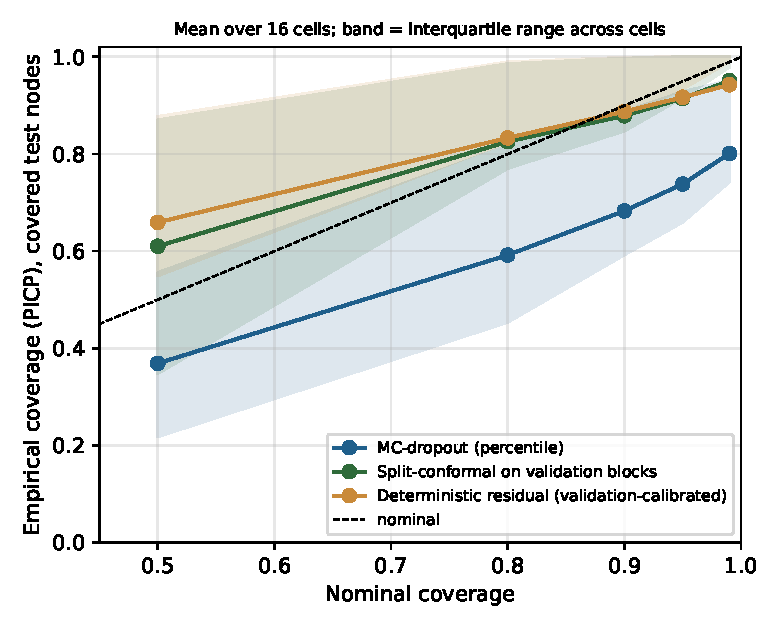
\includegraphics[width=\columnwidth]{novas/fig_calibracao_T14.pdf}
\caption{Prediction-interval coverage against nominal level under the spatially blocked protocol, by method, mean over the 16~cells with interquartile band.}
\label{fig:calibracao_T14}
\end{figure}

\subsection{Cross-city transfer}
\label{sec:cross_city_transfer}

Lins-trained seed-42 checkpoints are applied without fine-tuning to the blocked test partitions of Lins, Campinas, and Sorocaba (Table~\ref{tab:ood_blocked}); zeroing the topographic features raises mean RSSI MAE in every city tested, in-domain and out-of-domain alike, from \SI{0.399}{\deci\bel} to \SI{2.757}{\deci\bel} in Lins ($+$591.2\%), from \SI{1.353}{\deci\bel} to \SI{3.304}{\deci\bel} in Campinas ($+$144.1\%), and from \SI{1.622}{\deci\bel} to \SI{3.931}{\deci\bel} in Sorocaba ($+$142.4\%), with the percentage taken over the full-terrain arm. The same pattern holds at larger absolute magnitude on valid-target nodes for both RSSI and path loss, and the in-domain increase remains far larger than either out-of-domain city in both populations.

The reversal obtained in the preliminary experiment ($-$8 to $-$9\% out-of-domain) came from a different evaluation: it scored the entire 12.96-million-node graph of each quadrant, training and validation nodes included, rather than the held-out blocked test partition, which covers only about 6.3--6.4\% of that graph. Under the criterion fixed before this result, the blocked measurement confirms the qualitative pattern expected of a terrain-dependent model: the topographic advantage is positive everywhere and larger in-domain than out. The blocked measurement contradicts the earlier number, not this pattern, and the two are not comparable value by value.

\begin{table*}[t]
\caption{Cross-city transfer under the spatially blocked protocol (Section~\ref{sec:cross_city_transfer}): Lins checkpoints (seed~42, one per quadrant) on the blocked test partition of the same quadrant in Lins (in-domain), Campinas and Sorocaba. The no\_topo arm zeroes the eight topographic input features of the terrain nodes at inference. Entries are unweighted mean MAE over Q1--Q4 for all nodes (sentinel included), valid-target nodes for RSSI, and valid-target nodes for path loss (PL); $\Delta$ is no\_topo minus full, and the change is $\Delta$ divided by the full-arm MAE.}
\label{tab:ood_blocked}
\centering
\small
\setlength{\tabcolsep}{4pt}
\begin{tabular}{ll ccc ccc ccc}
\toprule
 & & \multicolumn{3}{c}{RSSI, all nodes} & \multicolumn{3}{c}{RSSI, valid-target} & \multicolumn{3}{c}{PL, valid-target} \\
\cmidrule(lr){3-5}\cmidrule(lr){6-8}\cmidrule(lr){9-11}
Target city & Arm & MAE (dB) & $\Delta$ (dB) & Change & MAE (dB) & $\Delta$ (dB) & Change & MAE (dB) & $\Delta$ (dB) & Change \\
\midrule
Lins (in-domain) & full & 0.399 & -- & -- & 3.92 & -- & -- & 3.64 & -- & -- \\
Lins (in-domain) & no\_topo & 2.757 & +2.358 & +591.2\% & 23.51 & +19.59 & +500.4\% & 29.98 & +26.34 & +722.6\% \\
\midrule
Campinas (OOD) & full & 1.353 & -- & -- & 5.73 & -- & -- & 7.54 & -- & -- \\
Campinas (OOD) & no\_topo & 3.304 & +1.950 & +144.1\% & 17.54 & +11.81 & +206.1\% & 25.02 & +17.48 & +231.9\% \\
\midrule
Sorocaba (OOD) & full & 1.622 & -- & -- & 7.50 & -- & -- & 8.72 & -- & -- \\
Sorocaba (OOD) & no\_topo & 3.931 & +2.309 & +142.4\% & 20.75 & +13.26 & +176.9\% & 27.45 & +18.72 & +214.7\% \\
\bottomrule
\end{tabular}
\end{table*}


\subsection{Computational cost}

Between GNN-RF and the graph-free control, the cost difference shows up as wall-clock time and memory. On Bauru, on the same GPU, GNN-RF trains in 3987\,s from scratch (Q1, 35 epochs) and 2323\,s under the transfer schedule (Q4, 20 epochs), with peak VRAM of 7475 and 7466\,MB, against 616\,s and 409\,s, with 653 and 676\,MB, for the graph-free control (Table~\ref{tab:cost}); these figures come from a single cell and a single seed. The accuracy gain over the graph-free control (Section~\ref{sec:robustness}) therefore comes at several times the training time and close to an order of magnitude more peak memory.

\begin{table}[!t]
\centering
\caption{Computational cost in the spatially blocked campaign (Bauru, seed~42): GNN-RF and the graph-free control (MLP, Section~\ref{sec:ablation_design}). Q1 trains from scratch (35 epochs); Q4 transfers (20 epochs). Size assumes 4 bytes per parameter and is given in MiB ($2^{20}$ bytes); peak VRAM is the maximum memory allocated by PyTorch during training and is given in MB ($10^{6}$ bytes).}
\label{tab:cost}
\setlength{\tabcolsep}{4pt}
\begin{tabular}{lrrrrrr}
\toprule
 & & & \multicolumn{2}{c}{Time (s)} & \multicolumn{2}{c}{Peak VRAM (MB)} \\
\cmidrule(lr){4-5}\cmidrule(lr){6-7}
Model & Params & Size (MiB) & Q1 & Q4 & Q1 & Q4 \\
\midrule
GNN-RF & \num{1812515} & 6.91 & 3987 & 2323 & 7475 & 7466 \\
MLP & \num{1812515} & 6.91 & 616 & 409 & 653 & 676 \\
\bottomrule
\end{tabular}
\end{table}



%% ====================================================================
\section{Discussion}
\label{sec:discussion}
%% ====================================================================

\subsection{Interpretation of results}

The structural ablation and the graph-free control bound what the terrain graph contributes on this reference, over two different scopes. In the eight Lins and Bauru cells of the ablation the trained model relies on its graph: damaging terrain-to-terrain edges costs more than damaging antenna-to-terrain edges in seven of the eight cells, and removing all edges costs accuracy except in Lins~Q1, where the empty graph barely changes the error (Section~\ref{sec:robustness}).

Across all four cities, GNN-RF is ahead of the graph-free control, but its city-level interval crosses zero and the cell-level result is sensitive to the inferential method (Section~\ref{sec:robustness}). In Bauru~Q1, the cell with the largest valid-target fraction (0.328), GNN-RF is ahead of the graph-free control in every training seed, an association between valid-target fraction and graph advantage that is exploratory, without an inferential test. This sample does not support generalizing a graph advantage to measured fields.

The node-wise adaptation receives the antenna-to-terrain relations of the graph and no terrain-to-terrain message, and with about one fifth of the parameters it has a lower valid-target RSSI MAE than the graph-free control (Section~\ref{sec:model_comparison}). Over the same nodes, its difference from GNN-RF is inconclusive relative to the pre-specified margin, so terrain-to-terrain message passing yields no detectable accuracy over what the node-wise adaptation already achieves. The structural ablation measures the cost of damaging the graph of a model trained with it, and the node-wise adaptation measures whether terrain-to-terrain messages are needed for accuracy.

Next to these learned controls, the comparison with empirical models survives calibration. Paired against the best calibrated model of each cell, GNN-RF has the lower error over all test nodes in 15 of the 16 cells (Section~\ref{sec:model_comparison}); over valid-target nodes the mean margin widens, and the four cells where GNN-RF trails are Campinas~Q2, Lins~Q1, Lins~Q2, and Sorocaba~Q2.

On strong-signal nodes near the serving transmitter, GNN-RF and the graph-free control underestimate RSSI. On valid-target nodes with target RSSI of at least $-$70~dBm, their node-weighted bias is $-$13.90 and $-$11.93\,dB, respectively, against $-$2.73\,dB for the node-wise adaptation; on those within 250\,m of the transmitter, it is $-$30.96 and $-$28.88\,dB, respectively, against $-$14.15\,dB. Within 2\,km of the transmitter, the least-squares slope of path loss against $\log_{10}$ of distance is 8.05\,dB per decade for GNN-RF and for the graph-free control and 23.22\,dB per decade for the node-wise adaptation, against 34.95\,dB per decade for the target, each a mean over the four cells with at least 50 such valid-target nodes (Bauru~Q1, Campinas~Q1, Campinas~Q3, and Lins~Q1). The reconstruction near the serving transmitter is the tightest limit of this study.

GNN-RF, the node-wise adaptation, and the graph-free control, the three networks sharing the output decoder, and GNN-RF retrained without any penalty term all place a smaller fraction of valid-target nodes below the free-space floor than the target itself (Table~\ref{tab:admissibility_blocked}). The monotonicity violation rate, in contrast, varies among networks trained with the same loss and decoder, so it is not set by them, and retraining without the penalty terms changes it only within an interval that contains zero. GNN-RF keeps its floor admissibility high but uneven across cities, clean in every Sorocaba run and in most Bauru and Lins runs, with more exceptions in Campinas.

The claims of this work rest on the blocked evaluation itself, on the joint reconstruction of path loss and RSSI in absolute decibels, and on controls that make the contribution of the graph measurable; the uncertainty evaluation adds a negative result, since no interval method tested reaches nominal per-cell coverage under spatial blocking. Free-space-floor admissibility is common to every network trained here on this target and satisfied almost everywhere by the target itself: it is verified on the outputs rather than credited to the graph.

Because the reference field is fully specified, the bench also measures the evaluation itself: the nearest-neighbor contrast of Section~\ref{sec:eval_protocol}, in line with the optimistic estimates that random cross-validation gives for spatially clustered data~\cite{meyer2021predicting}, separates spatial learning from partition leakage independently of where the labels come from, so the design can be reused unchanged with measured RSSI or drive-test path loss. The native 30\,m resolution of the Copernicus DEM (Section~\ref{sec:graph_construction}), however, bounds the achievable spatial granularity of the RF predictions.

\subsection{Methodological implications for RF emulation}

Within the scope of deterministic RF field emulation, the results suggest that sequential fine-tuning saves compute: continuing from an adjacent checkpoint for 20\,epochs shows no systematic difference from training from scratch for 35\,epochs (Section~\ref{sec:model_comparison}). They also suggest that, for surrogate emulation pipelines, terrain feature engineering weighs more than the one architectural contrast measured here, GNN-RF against a graph-free control, since zero-shot checkpoints transferred to unseen cities, tested on a single seed, suffer more from ablating topography than from the domain shift itself (Section~\ref{sec:cross_city_transfer}). Neither takeaway prescribes physical network deployment, which remains conditional on empirical field validation as detailed below.

\subsection{Simulation-derived targets and validity bounds}

A fundamental constraint of this study is that all target labels come from the deterministic propagation generator of Section~\ref{sec:methodology}, which computes path loss, RSSI, and coverage from antenna parameters, node-level terrain and vegetation features, and empirical correction factors without tracing terrain profiles. The reported MAE values (\SI{0.395}{\deci\bel} on all blocked test nodes) therefore represent reconstruction fidelity relative to these simulation outputs, not prediction accuracy against physical RF measurements.

The generator also omits mechanisms that a full link-level simulation would include: diffraction over real obstacles, Fresnel-zone clearance, line-of-sight testing, and multipath or ground-reflection effects are absent, and the knife-edge channel uses a single midpoint obstacle rather than the profile maximum. Its two-term link budget carries no noise floor, receiver noise figure, interference from neighboring cells, or SINR calculation, and coverage adds no fading margin, outage probability, shadowing standard deviation, or receiver sensitivity, remaining a hard threshold on the link budget rather than a link-quality decision. The generator draws no random term, so no log-normal shadowing is present; the uniform slope draw of the early pipeline was replaced by the DEM slope.

Both empirical base-loss models also run partly outside their validated range. The accuracy figures therefore bound fidelity to this extrapolated field, not agreement with Okumura--Hata or COST\,231 inside their original envelopes.

The gap between simulated and measured propagation in the Brazilian context is not quantified in this work, and studies that compare sub-GHz path-loss predictions with field measurements, in Cartagena, Spain~\cite{lorentelpez2026machine} and in the Amazon~\cite{lima2024lora}, report errors larger than the sub-decibel reconstruction figures obtained here. Validation against even partial field measurement data would be required before any operational use.

All evaluations are restricted to four cities in S\~{a}o Paulo state (Brazil), and generalization to other biomes, frequency bands, or network topologies has not been tested. The edge ablation covers only Lins and Bauru, whereas the graph-free control spans all four cities; the uncertainty evaluation covers all 16 cells but is limited to the seed-42 checkpoints, each sampled with 50 Monte Carlo passes.

The 2\,km exclusion buffer is narrower than the spatial autocorrelation range~\cite{valavi2019blockcv} of the reference field, measured at 20\,km in Lins and 30\,km in Bauru and not measured in the other two cities, so the blocked results retain some dependence between training and test. Buffering against the full 20--30\,km range is geometrically infeasible within quadrant-scale tiles. The 2\,km buffer suppresses immediate mesh-scale interpolation, as the order-of-magnitude error inflation of the nearest-neighbor baseline in Section~\ref{sec:eval_protocol} reflects, but residual regional autocorrelation remains an explicit bound on claim independence.

In three Sorocaba cells, 0.03--0.06\% of nodes with a valid target carry an RSSI below $-$150\,dBm that the target post-processing did not impute, and correcting Q3, the only one of these cells where it changes test error, in both arms does not change the conclusion of the comparison against the graph-free control in Section~\ref{sec:robustness} (the 16-cell aggregate moves from \SI{-0.2475}{\deci\bel} to \SI{-0.2431}{\deci\bel}, $p{=}0.0402$).

\subsection{Limitations and future directions}

The blocked cross-city results, in which zeroing topographic features hurts accuracy everywhere and more inside the training domain than outside it, motivate domain adaptation that preserves that terrain dependence when transferring across cities without full fine-tuning. Transfer of a radio-map model between indoor environments has relied on fine-tuning the whole network~\cite{jaiswal2026data}, whereas unsupervised domain adaptation guided by geographic coordinates already serves remote-sensing segmentation~\cite{marsocci2023geomultitasknet}. Interval methods that account for the non-exchangeability of spatial blocks are also needed, since split-conformal calibration on separate blocks did not transfer here (Table~\ref{tab:uncertainty_blocked}) and conformal coverage is no longer guaranteed once exchangeability is violated~\cite{zargarbashi2023conformal}.


%% ====================================================================
\section{Conclusions}
\label{sec:conclusions}
%% ====================================================================

This paper evaluates GNN-RF under a spatially blocked protocol because partition choice changes what a radio-map estimator's accuracy can support: a nearest-neighbor copy that fails under blocking looks adequate under a random node split in all 16 city--quadrant cells, and a geographic-split control on a RadioUNet adaptation from a preliminary experiment (Section~\ref{sec:eval_protocol}) failed in half of the same cells.

Under that blocked protocol, across all 16 cells (80~runs), GNN-RF reconstructs path loss and RSSI in absolute decibels, and coverage, over large-scale terrain graphs ($12.96 \times 10^6$~nodes), with a test RSSI MAE of \SI{0.395}{\deci\bel} (95\% CI [\num{0.309}, \num{0.480}], all test nodes). Paired against the best calibrated empirical model of each cell, it wins by a mean of \SI{0.746}{\deci\bel} ($p{=}2.59\times10^{-4}$) in 15 of the 16 cells and loses by \SI{0.009}{\deci\bel} in Campinas~Q2, and the margin widens on valid-target nodes. Its outputs stay within their activation ranges, and the fraction of valid-target nodes whose predicted path loss falls below the free-space floor of the serving transmitter is $1.39\times10^{-4}$, below the $2.43\times10^{-4}$ of the target itself.

The accuracy advantage over the graph-free control follows the antenna-to-terrain relations of the graph. On valid-target nodes, the two learners that receive the antenna-to-terrain relations of the graph, GNN-RF and the node-wise adaptation of RadioUNet, reach RSSI MAE of 2.0122 and 1.2327\,dB, below both the graph-free control matched in nominal parameters (2.7387\,dB) and the best calibrated empirical model of each cell (4.3624\,dB). Damaging the graph degrades the trained model on the eight Lins and Bauru cells, by \SI{1.72}{\deci\bel} on average when all edges are removed, except in Lins~Q1, where the empty graph leaves the error nearly unchanged.

Neither the terrain-to-terrain messages nor the penalty terms account for a resolvable part of that accuracy: the difference between the node-wise adaptation and GNN-RF is inconclusive relative to the pre-specified margin, and so are the differences of GNN-RF retrained without all four penalty terms or without the monotonicity term alone. Free-space-floor admissibility is common to every network trained here on this target and satisfied almost everywhere by the target itself, so it is not a contribution of the graph.

Training each quadrant from scratch shows no systematic advantage for the transfer chain, and under the same blocked protocol, zeroing topographic features raises cross-city error everywhere, more inside the training domain than outside it. The uncertainty evaluation is a negative result: under spatial blocking, neither MC Dropout nor its split-conformal correction reaches nominal coverage per cell, and a residual-based interval covers as much at no extra cost.

Future work will prioritize validation against field RF measurements to quantify the gap between simulation-derived reconstruction accuracy and physical-world prediction error. A wider exclusion buffer, non-sequential transfer strategies, and other frequency bands and regions beyond S\~{a}o Paulo state would extend the evaluation, and coupling DEM super-resolution, for which learned methods already exist~\cite{guo2025multi,cai2025jspsr}, with RF reconstruction in end-to-end pipelines is a further direction that the released benchmark makes testable.


%% ====================================================================
\section*{Acknowledgment}
%The authors gratefully acknowledge the Military Institute of Engineering for supporting and hosting this project. 
%% ====================================================================
%\section*{Declaration of Generative AI Use}
\textit{Declaration of Generative AI Use:} During the preparation of this work the authors used Claude (Anthropic) to assist with manuscript drafting, revision, and code development, and Gemini (Google) to support literature search. After using these tools, the authors reviewed and edited the content as needed and take full responsibility for the content of the published article.


%% ====================================================================
\section*{Conflict of Interest}
%% ====================================================================

The authors declare no conflicts of interest regarding this work.


%% ====================================================================
\section*{Data Availability}
%% ====================================================================

The target generator and the target corrector, identified by SHA-256 digest in the Supplementary Material, the $16\times3$ partition masks with their hashes and a verifier, the evaluation and baseline scripts, the training scripts, and 400~run logs, 400~checkpoints, and 400~prediction files, 80 each for GNN-RF, the graph-free control, the two retrained arms, and the node-wise adaptation, are available at \url{https://doi.org/10.5281/zenodo.23377937}~\pend{DOI publicado}. The 16~reference fields are not in the deposit: they are identified by SHA-256 digest and can be regenerated with the released generator and the public inputs. The complete generator specification is published as Supplementary Material.





\bibliographystyle{IEEEtran}
\bibliography{reference_R4min}

%% --- Biografias dos autores (IEEE Access) ---
%% Descomente e preencha. Requer arquivos de foto (ex.: seelig.png, salles.png)
%% com 1in x 1.25in. Para submissao inicial, biografias podem ser omitidas.
%
\begin{IEEEbiography}[{\includegraphics[width=1in,height=1.25in,clip,keepaspectratio]{seeling.png}}]{Luis Felipe Comodo Seelig} received the B.S. degree in Military Sciences from the Academia Militar das Agulhas Negras (AMAN), Resende, Brazil. He holds postgraduate specializations in Military Sciences from the Escola de Aperfeiçoamento de Oficiais do Exército (EsAO), Rio de Janeiro, Brazil; in Geoprocessing from the Universidade Federal do ABC (UFABC), Santo André, Brazil; and in Artificial Intelligence from the Universidade Tecnológica Federal do Paraná (UTFPR), Brazil. He also holds an MBA in Data Science and Analytics from the Universidade de São Paulo (USP), Brazil. He is currently a research student in the Defense Engineering Program at the Military Institute of Engineering (IME), Rio de Janeiro, Brazil, and a Research Associate with the Laboratório de Ciências Militares (LCM), Escola de Comando e Estado-Maior do Exército (ECEME), Rio de Janeiro, Brazil.
His current research interests include graph neural networks applied to geospatial intelligence, remote sensing classification and super-resolution, military decision-support systems, and radio-frequency propagation modeling.
% Biografia do primeiro autor.
\end{IEEEbiography}
%
% \begin{IEEEbiography}[{\includegraphics[width=1in,height=1.25in,clip,keepaspectratio]{salles.png}}]{R. M. Salles}
% Biografia do segundo autor.
% \end{IEEEbiography}

\begin{IEEEbiography}[{\includegraphics[width=1in,height=1.25in,clip,keepaspectratio]{salles.png}}]{Ronaldo Moreira Salles} received the B.Sc. degree in Electronic Engineering from the Military Institute of Engineering (IME), Brazil, in 1992, the M.Sc. degree in Systems and Computing from IME in 1998, and the Ph.D. degree in Computer Science (Computer Networks) from Imperial College London, U.K., in 2004.
He is currently an Associate Professor at the Polytechnic Institute of Porto (ESTG), Portugal, and a researcher at CIICESI (Center for Innovation and Research in Business Sciences and Information Systems). He is also a professor with the Military Institute of Engineering, Brazil, contributing to graduate programs in Computer Science and Defense Engineering.
His research interests include cybersecurity, computer networks, network security, performance evaluation, graph neural networks, remote sensing, system modeling and simulation, optimization and stochastic processes.
Dr. Salles has extensive experience in both academic research and applied projects in defense and critical infrastructures. He has coordinated and participated in multiple research initiatives in cyber defense and network security and has contributed to high-impact publications in leading journals and conferences.
\end{IEEEbiography}


\EOD

\end{document}
